\documentclass[twoside]{book}

% Packages required by doxygen
\usepackage{fixltx2e}
\usepackage{calc}
\usepackage{doxygen}
\usepackage[export]{adjustbox} % also loads graphicx
\usepackage{graphicx}
\usepackage[utf8]{inputenc}
\usepackage{makeidx}
\usepackage{multicol}
\usepackage{multirow}
\PassOptionsToPackage{warn}{textcomp}
\usepackage{textcomp}
\usepackage[nointegrals]{wasysym}
\usepackage[table]{xcolor}

% NLS support packages
\usepackage[french]{babel}

% Font selection
\usepackage[T1]{fontenc}
\usepackage[scaled=.90]{helvet}
\usepackage{courier}
\usepackage{amssymb}
\usepackage{sectsty}
\renewcommand{\familydefault}{\sfdefault}
\allsectionsfont{%
  \fontseries{bc}\selectfont%
  \color{darkgray}%
}
\renewcommand{\DoxyLabelFont}{%
  \fontseries{bc}\selectfont%
  \color{darkgray}%
}
\newcommand{\+}{\discretionary{\mbox{\scriptsize$\hookleftarrow$}}{}{}}

% Page & text layout
\usepackage{geometry}
\geometry{%
  a4paper,%
  top=2.5cm,%
  bottom=2.5cm,%
  left=2.5cm,%
  right=2.5cm%
}
\tolerance=750
\hfuzz=15pt
\hbadness=750
\setlength{\emergencystretch}{15pt}
\setlength{\parindent}{0cm}
\setlength{\parskip}{3ex plus 2ex minus 2ex}
\makeatletter
\renewcommand{\paragraph}{%
  \@startsection{paragraph}{4}{0ex}{-1.0ex}{1.0ex}{%
    \normalfont\normalsize\bfseries\SS@parafont%
  }%
}
\renewcommand{\subparagraph}{%
  \@startsection{subparagraph}{5}{0ex}{-1.0ex}{1.0ex}{%
    \normalfont\normalsize\bfseries\SS@subparafont%
  }%
}
\makeatother

% Headers & footers
\usepackage{fancyhdr}
\pagestyle{fancyplain}
\fancyhead[LE]{\fancyplain{}{\bfseries\thepage}}
\fancyhead[CE]{\fancyplain{}{}}
\fancyhead[RE]{\fancyplain{}{\bfseries\leftmark}}
\fancyhead[LO]{\fancyplain{}{\bfseries\rightmark}}
\fancyhead[CO]{\fancyplain{}{}}
\fancyhead[RO]{\fancyplain{}{\bfseries\thepage}}
\fancyfoot[LE]{\fancyplain{}{}}
\fancyfoot[CE]{\fancyplain{}{}}
\fancyfoot[RE]{\fancyplain{}{\bfseries\scriptsize Généré par Doxygen }}
\fancyfoot[LO]{\fancyplain{}{\bfseries\scriptsize Généré par Doxygen }}
\fancyfoot[CO]{\fancyplain{}{}}
\fancyfoot[RO]{\fancyplain{}{}}
\renewcommand{\footrulewidth}{0.4pt}
\renewcommand{\chaptermark}[1]{%
  \markboth{#1}{}%
}
\renewcommand{\sectionmark}[1]{%
  \markright{\thesection\ #1}%
}

% Indices & bibliography
\usepackage{natbib}
\usepackage[titles]{tocloft}
\setcounter{tocdepth}{3}
\setcounter{secnumdepth}{5}
\makeindex

% Hyperlinks (required, but should be loaded last)
\usepackage{ifpdf}
\ifpdf
  \usepackage[pdftex,pagebackref=true]{hyperref}
\else
  \usepackage[ps2pdf,pagebackref=true]{hyperref}
\fi
\hypersetup{%
  colorlinks=true,%
  linkcolor=blue,%
  citecolor=blue,%
  unicode%
}

% Custom commands
\newcommand{\clearemptydoublepage}{%
  \newpage{\pagestyle{empty}\cleardoublepage}%
}

\usepackage{caption}
\captionsetup{labelsep=space,justification=centering,font={bf},singlelinecheck=off,skip=4pt,position=top}

%===== C O N T E N T S =====

\begin{document}

% Titlepage & ToC
\hypersetup{pageanchor=false,
             bookmarksnumbered=true,
             pdfencoding=unicode
            }
\pagenumbering{alph}
\begin{titlepage}
\vspace*{7cm}
\begin{center}%
{\Large Mini-\/Éditeur }\\
\vspace*{1cm}
{\large Généré par Doxygen 1.8.13}\\
\end{center}
\end{titlepage}
\clearemptydoublepage
\pagenumbering{roman}
\tableofcontents
\clearemptydoublepage
\pagenumbering{arabic}
\hypersetup{pageanchor=true}

%--- Begin generated contents ---
\chapter{Index des espaces de nommage}
\section{Paquetages}
Liste des paquetages avec une brève description (si disponible) \+:\begin{DoxyCompactList}
\item\contentsline{section}{\hyperlink{namespacefr_1_1istic_1_1m1_1_1aco_1_1miniediteur_1_1v1}{fr.\+istic.\+m1.\+aco.\+miniediteur.\+v1} }{\pageref{namespacefr_1_1istic_1_1m1_1_1aco_1_1miniediteur_1_1v1}}{}
\end{DoxyCompactList}

\chapter{Index hiérarchique}
\section{Hiérarchie des classes}
Cette liste d\textquotesingle{}héritage est classée approximativement par ordre alphabétique \+:\begin{DoxyCompactList}
\item \contentsline{section}{fr.\+istic.\+m1.\+aco.\+miniediteur.\+v1.\+Buffer}{\pageref{classfr_1_1istic_1_1m1_1_1aco_1_1miniediteur_1_1v1_1_1Buffer}}{}
\item \contentsline{section}{fr.\+istic.\+m1.\+aco.\+miniediteur.\+v1.\+Commande}{\pageref{interfacefr_1_1istic_1_1m1_1_1aco_1_1miniediteur_1_1v1_1_1Commande}}{}
\begin{DoxyCompactList}
\item \contentsline{section}{fr.\+istic.\+m1.\+aco.\+miniediteur.\+v1.\+Coller}{\pageref{classfr_1_1istic_1_1m1_1_1aco_1_1miniediteur_1_1v1_1_1Coller}}{}
\item \contentsline{section}{fr.\+istic.\+m1.\+aco.\+miniediteur.\+v1.\+Copier}{\pageref{classfr_1_1istic_1_1m1_1_1aco_1_1miniediteur_1_1v1_1_1Copier}}{}
\item \contentsline{section}{fr.\+istic.\+m1.\+aco.\+miniediteur.\+v1.\+Couper}{\pageref{classfr_1_1istic_1_1m1_1_1aco_1_1miniediteur_1_1v1_1_1Couper}}{}
\item \contentsline{section}{fr.\+istic.\+m1.\+aco.\+miniediteur.\+v1.\+Defaire}{\pageref{classfr_1_1istic_1_1m1_1_1aco_1_1miniediteur_1_1v1_1_1Defaire}}{}
\item \contentsline{section}{fr.\+istic.\+m1.\+aco.\+miniediteur.\+v1.\+Demarrer}{\pageref{classfr_1_1istic_1_1m1_1_1aco_1_1miniediteur_1_1v1_1_1Demarrer}}{}
\item \contentsline{section}{fr.\+istic.\+m1.\+aco.\+miniediteur.\+v1.\+Inserer}{\pageref{classfr_1_1istic_1_1m1_1_1aco_1_1miniediteur_1_1v1_1_1Inserer}}{}
\item \contentsline{section}{fr.\+istic.\+m1.\+aco.\+miniediteur.\+v1.\+Refaire}{\pageref{classfr_1_1istic_1_1m1_1_1aco_1_1miniediteur_1_1v1_1_1Refaire}}{}
\item \contentsline{section}{fr.\+istic.\+m1.\+aco.\+miniediteur.\+v1.\+Rejouer}{\pageref{classfr_1_1istic_1_1m1_1_1aco_1_1miniediteur_1_1v1_1_1Rejouer}}{}
\item \contentsline{section}{fr.\+istic.\+m1.\+aco.\+miniediteur.\+v1.\+Selectionner}{\pageref{classfr_1_1istic_1_1m1_1_1aco_1_1miniediteur_1_1v1_1_1Selectionner}}{}
\item \contentsline{section}{fr.\+istic.\+m1.\+aco.\+miniediteur.\+v1.\+Stopper}{\pageref{classfr_1_1istic_1_1m1_1_1aco_1_1miniediteur_1_1v1_1_1Stopper}}{}
\end{DoxyCompactList}
\item \contentsline{section}{fr.\+istic.\+m1.\+aco.\+miniediteur.\+v1.\+Editeur}{\pageref{classfr_1_1istic_1_1m1_1_1aco_1_1miniediteur_1_1v1_1_1Editeur}}{}
\item \contentsline{section}{fr.\+istic.\+m1.\+aco.\+miniediteur.\+v1.\+Enregistrable}{\pageref{interfacefr_1_1istic_1_1m1_1_1aco_1_1miniediteur_1_1v1_1_1Enregistrable}}{}
\begin{DoxyCompactList}
\item \contentsline{section}{fr.\+istic.\+m1.\+aco.\+miniediteur.\+v1.\+Coller}{\pageref{classfr_1_1istic_1_1m1_1_1aco_1_1miniediteur_1_1v1_1_1Coller}}{}
\item \contentsline{section}{fr.\+istic.\+m1.\+aco.\+miniediteur.\+v1.\+Copier}{\pageref{classfr_1_1istic_1_1m1_1_1aco_1_1miniediteur_1_1v1_1_1Copier}}{}
\item \contentsline{section}{fr.\+istic.\+m1.\+aco.\+miniediteur.\+v1.\+Couper}{\pageref{classfr_1_1istic_1_1m1_1_1aco_1_1miniediteur_1_1v1_1_1Couper}}{}
\item \contentsline{section}{fr.\+istic.\+m1.\+aco.\+miniediteur.\+v1.\+Inserer}{\pageref{classfr_1_1istic_1_1m1_1_1aco_1_1miniediteur_1_1v1_1_1Inserer}}{}
\item \contentsline{section}{fr.\+istic.\+m1.\+aco.\+miniediteur.\+v1.\+Selectionner}{\pageref{classfr_1_1istic_1_1m1_1_1aco_1_1miniediteur_1_1v1_1_1Selectionner}}{}
\end{DoxyCompactList}
\item \contentsline{section}{fr.\+istic.\+m1.\+aco.\+miniediteur.\+v1.\+Enregistreur}{\pageref{interfacefr_1_1istic_1_1m1_1_1aco_1_1miniediteur_1_1v1_1_1Enregistreur}}{}
\item \contentsline{section}{fr.\+istic.\+m1.\+aco.\+miniediteur.\+v1.\+Gestionnaire\+Defaire\+Refaire}{\pageref{interfacefr_1_1istic_1_1m1_1_1aco_1_1miniediteur_1_1v1_1_1GestionnaireDefaireRefaire}}{}
\item \contentsline{section}{fr.\+istic.\+m1.\+aco.\+miniediteur.\+v1.\+I\+HM}{\pageref{interfacefr_1_1istic_1_1m1_1_1aco_1_1miniediteur_1_1v1_1_1IHM}}{}
\item \contentsline{section}{fr.\+istic.\+m1.\+aco.\+miniediteur.\+v1.\+Memento}{\pageref{interfacefr_1_1istic_1_1m1_1_1aco_1_1miniediteur_1_1v1_1_1Memento}}{}
\begin{DoxyCompactList}
\item \contentsline{section}{fr.\+istic.\+m1.\+aco.\+miniediteur.\+v1.\+Memento\+Inserer}{\pageref{classfr_1_1istic_1_1m1_1_1aco_1_1miniediteur_1_1v1_1_1MementoInserer}}{}
\item \contentsline{section}{fr.\+istic.\+m1.\+aco.\+miniediteur.\+v1.\+Memento\+Selectionner}{\pageref{classfr_1_1istic_1_1m1_1_1aco_1_1miniediteur_1_1v1_1_1MementoSelectionner}}{}
\end{DoxyCompactList}
\item \contentsline{section}{fr.\+istic.\+m1.\+aco.\+miniediteur.\+v1.\+Moteur}{\pageref{interfacefr_1_1istic_1_1m1_1_1aco_1_1miniediteur_1_1v1_1_1Moteur}}{}
\begin{DoxyCompactList}
\item \contentsline{section}{fr.\+istic.\+m1.\+aco.\+miniediteur.\+v1.\+Impl\+Moteur}{\pageref{classfr_1_1istic_1_1m1_1_1aco_1_1miniediteur_1_1v1_1_1ImplMoteur}}{}
\end{DoxyCompactList}
\item \contentsline{section}{fr.\+istic.\+m1.\+aco.\+miniediteur.\+v1.\+Presse\+Papier}{\pageref{classfr_1_1istic_1_1m1_1_1aco_1_1miniediteur_1_1v1_1_1PressePapier}}{}
\item \contentsline{section}{fr.\+istic.\+m1.\+aco.\+miniediteur.\+v1.\+Selection}{\pageref{classfr_1_1istic_1_1m1_1_1aco_1_1miniediteur_1_1v1_1_1Selection}}{}
\end{DoxyCompactList}

\chapter{Index des classes}
\section{Liste des classes}
Liste des classes, structures, unions et interfaces avec une brève description \+:\begin{DoxyCompactList}
\item\contentsline{section}{\hyperlink{classfr_1_1istic_1_1m1_1_1aco_1_1miniediteur_1_1v1_1_1Buffer}{fr.\+istic.\+m1.\+aco.\+miniediteur.\+v1.\+Buffer} }{\pageref{classfr_1_1istic_1_1m1_1_1aco_1_1miniediteur_1_1v1_1_1Buffer}}{}
\item\contentsline{section}{\hyperlink{classfr_1_1istic_1_1m1_1_1aco_1_1miniediteur_1_1v1_1_1Coller}{fr.\+istic.\+m1.\+aco.\+miniediteur.\+v1.\+Coller} \\*Classe contrôlant le fonctionnement de la fonctionnalité permettant de \hyperlink{classfr_1_1istic_1_1m1_1_1aco_1_1miniediteur_1_1v1_1_1Coller}{Coller} dans un \char`\"{}copié-\/collé\char`\"{} }{\pageref{classfr_1_1istic_1_1m1_1_1aco_1_1miniediteur_1_1v1_1_1Coller}}{}
\item\contentsline{section}{\hyperlink{interfacefr_1_1istic_1_1m1_1_1aco_1_1miniediteur_1_1v1_1_1Commande}{fr.\+istic.\+m1.\+aco.\+miniediteur.\+v1.\+Commande} \\*Interface décrivant une commande déclenchée par une action sur l\textquotesingle{}\hyperlink{interfacefr_1_1istic_1_1m1_1_1aco_1_1miniediteur_1_1v1_1_1IHM}{I\+HM} de l\textquotesingle{}Utilisateur }{\pageref{interfacefr_1_1istic_1_1m1_1_1aco_1_1miniediteur_1_1v1_1_1Commande}}{}
\item\contentsline{section}{\hyperlink{classfr_1_1istic_1_1m1_1_1aco_1_1miniediteur_1_1v1_1_1Copier}{fr.\+istic.\+m1.\+aco.\+miniediteur.\+v1.\+Copier} \\*Classe contrôlant le fonctionnement de la fonctionnalité permettant de \hyperlink{classfr_1_1istic_1_1m1_1_1aco_1_1miniediteur_1_1v1_1_1Copier}{Copier} dans un \char`\"{}copié-\/collé\char`\"{} }{\pageref{classfr_1_1istic_1_1m1_1_1aco_1_1miniediteur_1_1v1_1_1Copier}}{}
\item\contentsline{section}{\hyperlink{classfr_1_1istic_1_1m1_1_1aco_1_1miniediteur_1_1v1_1_1Couper}{fr.\+istic.\+m1.\+aco.\+miniediteur.\+v1.\+Couper} }{\pageref{classfr_1_1istic_1_1m1_1_1aco_1_1miniediteur_1_1v1_1_1Couper}}{}
\item\contentsline{section}{\hyperlink{classfr_1_1istic_1_1m1_1_1aco_1_1miniediteur_1_1v1_1_1Defaire}{fr.\+istic.\+m1.\+aco.\+miniediteur.\+v1.\+Defaire} }{\pageref{classfr_1_1istic_1_1m1_1_1aco_1_1miniediteur_1_1v1_1_1Defaire}}{}
\item\contentsline{section}{\hyperlink{classfr_1_1istic_1_1m1_1_1aco_1_1miniediteur_1_1v1_1_1Demarrer}{fr.\+istic.\+m1.\+aco.\+miniediteur.\+v1.\+Demarrer} }{\pageref{classfr_1_1istic_1_1m1_1_1aco_1_1miniediteur_1_1v1_1_1Demarrer}}{}
\item\contentsline{section}{\hyperlink{classfr_1_1istic_1_1m1_1_1aco_1_1miniediteur_1_1v1_1_1Editeur}{fr.\+istic.\+m1.\+aco.\+miniediteur.\+v1.\+Editeur} }{\pageref{classfr_1_1istic_1_1m1_1_1aco_1_1miniediteur_1_1v1_1_1Editeur}}{}
\item\contentsline{section}{\hyperlink{interfacefr_1_1istic_1_1m1_1_1aco_1_1miniediteur_1_1v1_1_1Enregistrable}{fr.\+istic.\+m1.\+aco.\+miniediteur.\+v1.\+Enregistrable} }{\pageref{interfacefr_1_1istic_1_1m1_1_1aco_1_1miniediteur_1_1v1_1_1Enregistrable}}{}
\item\contentsline{section}{\hyperlink{interfacefr_1_1istic_1_1m1_1_1aco_1_1miniediteur_1_1v1_1_1Enregistreur}{fr.\+istic.\+m1.\+aco.\+miniediteur.\+v1.\+Enregistreur} }{\pageref{interfacefr_1_1istic_1_1m1_1_1aco_1_1miniediteur_1_1v1_1_1Enregistreur}}{}
\item\contentsline{section}{\hyperlink{interfacefr_1_1istic_1_1m1_1_1aco_1_1miniediteur_1_1v1_1_1GestionnaireDefaireRefaire}{fr.\+istic.\+m1.\+aco.\+miniediteur.\+v1.\+Gestionnaire\+Defaire\+Refaire} }{\pageref{interfacefr_1_1istic_1_1m1_1_1aco_1_1miniediteur_1_1v1_1_1GestionnaireDefaireRefaire}}{}
\item\contentsline{section}{\hyperlink{interfacefr_1_1istic_1_1m1_1_1aco_1_1miniediteur_1_1v1_1_1IHM}{fr.\+istic.\+m1.\+aco.\+miniediteur.\+v1.\+I\+HM} }{\pageref{interfacefr_1_1istic_1_1m1_1_1aco_1_1miniediteur_1_1v1_1_1IHM}}{}
\item\contentsline{section}{\hyperlink{classfr_1_1istic_1_1m1_1_1aco_1_1miniediteur_1_1v1_1_1ImplMoteur}{fr.\+istic.\+m1.\+aco.\+miniediteur.\+v1.\+Impl\+Moteur} }{\pageref{classfr_1_1istic_1_1m1_1_1aco_1_1miniediteur_1_1v1_1_1ImplMoteur}}{}
\item\contentsline{section}{\hyperlink{classfr_1_1istic_1_1m1_1_1aco_1_1miniediteur_1_1v1_1_1Inserer}{fr.\+istic.\+m1.\+aco.\+miniediteur.\+v1.\+Inserer} }{\pageref{classfr_1_1istic_1_1m1_1_1aco_1_1miniediteur_1_1v1_1_1Inserer}}{}
\item\contentsline{section}{\hyperlink{interfacefr_1_1istic_1_1m1_1_1aco_1_1miniediteur_1_1v1_1_1Memento}{fr.\+istic.\+m1.\+aco.\+miniediteur.\+v1.\+Memento} }{\pageref{interfacefr_1_1istic_1_1m1_1_1aco_1_1miniediteur_1_1v1_1_1Memento}}{}
\item\contentsline{section}{\hyperlink{classfr_1_1istic_1_1m1_1_1aco_1_1miniediteur_1_1v1_1_1MementoInserer}{fr.\+istic.\+m1.\+aco.\+miniediteur.\+v1.\+Memento\+Inserer} }{\pageref{classfr_1_1istic_1_1m1_1_1aco_1_1miniediteur_1_1v1_1_1MementoInserer}}{}
\item\contentsline{section}{\hyperlink{classfr_1_1istic_1_1m1_1_1aco_1_1miniediteur_1_1v1_1_1MementoSelectionner}{fr.\+istic.\+m1.\+aco.\+miniediteur.\+v1.\+Memento\+Selectionner} }{\pageref{classfr_1_1istic_1_1m1_1_1aco_1_1miniediteur_1_1v1_1_1MementoSelectionner}}{}
\item\contentsline{section}{\hyperlink{interfacefr_1_1istic_1_1m1_1_1aco_1_1miniediteur_1_1v1_1_1Moteur}{fr.\+istic.\+m1.\+aco.\+miniediteur.\+v1.\+Moteur} }{\pageref{interfacefr_1_1istic_1_1m1_1_1aco_1_1miniediteur_1_1v1_1_1Moteur}}{}
\item\contentsline{section}{\hyperlink{classfr_1_1istic_1_1m1_1_1aco_1_1miniediteur_1_1v1_1_1PressePapier}{fr.\+istic.\+m1.\+aco.\+miniediteur.\+v1.\+Presse\+Papier} }{\pageref{classfr_1_1istic_1_1m1_1_1aco_1_1miniediteur_1_1v1_1_1PressePapier}}{}
\item\contentsline{section}{\hyperlink{classfr_1_1istic_1_1m1_1_1aco_1_1miniediteur_1_1v1_1_1Refaire}{fr.\+istic.\+m1.\+aco.\+miniediteur.\+v1.\+Refaire} }{\pageref{classfr_1_1istic_1_1m1_1_1aco_1_1miniediteur_1_1v1_1_1Refaire}}{}
\item\contentsline{section}{\hyperlink{classfr_1_1istic_1_1m1_1_1aco_1_1miniediteur_1_1v1_1_1Rejouer}{fr.\+istic.\+m1.\+aco.\+miniediteur.\+v1.\+Rejouer} }{\pageref{classfr_1_1istic_1_1m1_1_1aco_1_1miniediteur_1_1v1_1_1Rejouer}}{}
\item\contentsline{section}{\hyperlink{classfr_1_1istic_1_1m1_1_1aco_1_1miniediteur_1_1v1_1_1Selection}{fr.\+istic.\+m1.\+aco.\+miniediteur.\+v1.\+Selection} }{\pageref{classfr_1_1istic_1_1m1_1_1aco_1_1miniediteur_1_1v1_1_1Selection}}{}
\item\contentsline{section}{\hyperlink{classfr_1_1istic_1_1m1_1_1aco_1_1miniediteur_1_1v1_1_1Selectionner}{fr.\+istic.\+m1.\+aco.\+miniediteur.\+v1.\+Selectionner} }{\pageref{classfr_1_1istic_1_1m1_1_1aco_1_1miniediteur_1_1v1_1_1Selectionner}}{}
\item\contentsline{section}{\hyperlink{classfr_1_1istic_1_1m1_1_1aco_1_1miniediteur_1_1v1_1_1Stopper}{fr.\+istic.\+m1.\+aco.\+miniediteur.\+v1.\+Stopper} }{\pageref{classfr_1_1istic_1_1m1_1_1aco_1_1miniediteur_1_1v1_1_1Stopper}}{}
\end{DoxyCompactList}

\chapter{Index des fichiers}
\section{Liste des fichiers}
Liste de tous les fichiers documentés avec une brève description \+:\begin{DoxyCompactList}
\item\contentsline{section}{src/fr/istic/m1/aco/miniediteur/v1/\hyperlink{Coller_8java}{Coller.\+java} }{\pageref{Coller_8java}}{}
\item\contentsline{section}{src/fr/istic/m1/aco/miniediteur/v1/\hyperlink{Commande_8java}{Commande.\+java} }{\pageref{Commande_8java}}{}
\item\contentsline{section}{src/fr/istic/m1/aco/miniediteur/v1/\hyperlink{Copier_8java}{Copier.\+java} }{\pageref{Copier_8java}}{}
\item\contentsline{section}{src/fr/istic/m1/aco/miniediteur/v1/\hyperlink{Couper_8java}{Couper.\+java} }{\pageref{Couper_8java}}{}
\item\contentsline{section}{src/fr/istic/m1/aco/miniediteur/v1/\hyperlink{Defaire_8java}{Defaire.\+java} }{\pageref{Defaire_8java}}{}
\item\contentsline{section}{src/fr/istic/m1/aco/miniediteur/v1/\hyperlink{Demarrer_8java}{Demarrer.\+java} }{\pageref{Demarrer_8java}}{}
\item\contentsline{section}{src/fr/istic/m1/aco/miniediteur/v1/\hyperlink{Enregistrable_8java}{Enregistrable.\+java} }{\pageref{Enregistrable_8java}}{}
\item\contentsline{section}{src/fr/istic/m1/aco/miniediteur/v1/\hyperlink{Enregistreur_8java}{Enregistreur.\+java} }{\pageref{Enregistreur_8java}}{}
\item\contentsline{section}{src/fr/istic/m1/aco/miniediteur/v1/\hyperlink{GestionnaireDefaireRefaire_8java}{Gestionnaire\+Defaire\+Refaire.\+java} }{\pageref{GestionnaireDefaireRefaire_8java}}{}
\item\contentsline{section}{src/fr/istic/m1/aco/miniediteur/v1/\hyperlink{IHM_8java}{I\+H\+M.\+java} }{\pageref{IHM_8java}}{}
\item\contentsline{section}{src/fr/istic/m1/aco/miniediteur/v1/\hyperlink{Inserer_8java}{Inserer.\+java} }{\pageref{Inserer_8java}}{}
\end{DoxyCompactList}

\chapter{Documentation des espaces de nommage}
\hypertarget{namespacefr_1_1istic_1_1m1_1_1aco_1_1miniediteur_1_1v1}{}\section{Paquetage fr.\+istic.\+m1.\+aco.\+miniediteur.\+v1}
\label{namespacefr_1_1istic_1_1m1_1_1aco_1_1miniediteur_1_1v1}\index{fr.\+istic.\+m1.\+aco.\+miniediteur.\+v1@{fr.\+istic.\+m1.\+aco.\+miniediteur.\+v1}}
\subsection*{Classes}
\begin{DoxyCompactItemize}
\item 
class \hyperlink{classfr_1_1istic_1_1m1_1_1aco_1_1miniediteur_1_1v1_1_1Buffer}{Buffer}
\item 
class \hyperlink{classfr_1_1istic_1_1m1_1_1aco_1_1miniediteur_1_1v1_1_1Coller}{Coller}
\begin{DoxyCompactList}\small\item\em Classe contrôlant le fonctionnement de la fonctionnalité permettant de \hyperlink{classfr_1_1istic_1_1m1_1_1aco_1_1miniediteur_1_1v1_1_1Coller}{Coller} dans un \char`\"{}copié-\/collé\char`\"{}. \end{DoxyCompactList}\item 
interface \hyperlink{interfacefr_1_1istic_1_1m1_1_1aco_1_1miniediteur_1_1v1_1_1Commande}{Commande}
\begin{DoxyCompactList}\small\item\em Interface décrivant une commande déclenchée par une action sur l\textquotesingle{}\hyperlink{interfacefr_1_1istic_1_1m1_1_1aco_1_1miniediteur_1_1v1_1_1IHM}{I\+HM} de l\textquotesingle{}Utilisateur. \end{DoxyCompactList}\item 
class \hyperlink{classfr_1_1istic_1_1m1_1_1aco_1_1miniediteur_1_1v1_1_1Copier}{Copier}
\begin{DoxyCompactList}\small\item\em Classe contrôlant le fonctionnement de la fonctionnalité permettant de \hyperlink{classfr_1_1istic_1_1m1_1_1aco_1_1miniediteur_1_1v1_1_1Copier}{Copier} dans un \char`\"{}copié-\/collé\char`\"{}. \end{DoxyCompactList}\item 
class \hyperlink{classfr_1_1istic_1_1m1_1_1aco_1_1miniediteur_1_1v1_1_1Couper}{Couper}
\item 
class \hyperlink{classfr_1_1istic_1_1m1_1_1aco_1_1miniediteur_1_1v1_1_1Defaire}{Defaire}
\item 
class \hyperlink{classfr_1_1istic_1_1m1_1_1aco_1_1miniediteur_1_1v1_1_1Demarrer}{Demarrer}
\item 
class \hyperlink{classfr_1_1istic_1_1m1_1_1aco_1_1miniediteur_1_1v1_1_1Editeur}{Editeur}
\item 
interface \hyperlink{interfacefr_1_1istic_1_1m1_1_1aco_1_1miniediteur_1_1v1_1_1Enregistrable}{Enregistrable}
\item 
interface \hyperlink{interfacefr_1_1istic_1_1m1_1_1aco_1_1miniediteur_1_1v1_1_1Enregistreur}{Enregistreur}
\item 
interface \hyperlink{interfacefr_1_1istic_1_1m1_1_1aco_1_1miniediteur_1_1v1_1_1GestionnaireDefaireRefaire}{Gestionnaire\+Defaire\+Refaire}
\item 
interface \hyperlink{interfacefr_1_1istic_1_1m1_1_1aco_1_1miniediteur_1_1v1_1_1IHM}{I\+HM}
\item 
class \hyperlink{classfr_1_1istic_1_1m1_1_1aco_1_1miniediteur_1_1v1_1_1ImplMoteur}{Impl\+Moteur}
\item 
class \hyperlink{classfr_1_1istic_1_1m1_1_1aco_1_1miniediteur_1_1v1_1_1Inserer}{Inserer}
\item 
interface \hyperlink{interfacefr_1_1istic_1_1m1_1_1aco_1_1miniediteur_1_1v1_1_1Memento}{Memento}
\item 
class \hyperlink{classfr_1_1istic_1_1m1_1_1aco_1_1miniediteur_1_1v1_1_1MementoInserer}{Memento\+Inserer}
\item 
class \hyperlink{classfr_1_1istic_1_1m1_1_1aco_1_1miniediteur_1_1v1_1_1MementoSelectionner}{Memento\+Selectionner}
\item 
interface \hyperlink{interfacefr_1_1istic_1_1m1_1_1aco_1_1miniediteur_1_1v1_1_1Moteur}{Moteur}
\item 
class \hyperlink{classfr_1_1istic_1_1m1_1_1aco_1_1miniediteur_1_1v1_1_1PressePapier}{Presse\+Papier}
\item 
class \hyperlink{classfr_1_1istic_1_1m1_1_1aco_1_1miniediteur_1_1v1_1_1Refaire}{Refaire}
\item 
class \hyperlink{classfr_1_1istic_1_1m1_1_1aco_1_1miniediteur_1_1v1_1_1Rejouer}{Rejouer}
\item 
class \hyperlink{classfr_1_1istic_1_1m1_1_1aco_1_1miniediteur_1_1v1_1_1Selection}{Selection}
\item 
class \hyperlink{classfr_1_1istic_1_1m1_1_1aco_1_1miniediteur_1_1v1_1_1Selectionner}{Selectionner}
\item 
class \hyperlink{classfr_1_1istic_1_1m1_1_1aco_1_1miniediteur_1_1v1_1_1Stopper}{Stopper}
\end{DoxyCompactItemize}


\subsection{Description détaillée}
@(\#) Editeur.\+java 
\chapter{Documentation des classes}
\hypertarget{classfr_1_1istic_1_1m1_1_1aco_1_1miniediteur_1_1v1_1_1Buffer}{}\section{Référence de la classe fr.\+istic.\+m1.\+aco.\+miniediteur.\+v1.\+Buffer}
\label{classfr_1_1istic_1_1m1_1_1aco_1_1miniediteur_1_1v1_1_1Buffer}\index{fr.\+istic.\+m1.\+aco.\+miniediteur.\+v1.\+Buffer@{fr.\+istic.\+m1.\+aco.\+miniediteur.\+v1.\+Buffer}}


\subsection{Description détaillée}
Created by 16009566 on 20/10/17. 

La documentation de cette classe a été générée à partir du fichier suivant \+:\begin{DoxyCompactItemize}
\item 
src/fr/istic/m1/aco/miniediteur/v1/Buffer.\+java\end{DoxyCompactItemize}

\hypertarget{classfr_1_1istic_1_1m1_1_1aco_1_1miniediteur_1_1v1_1_1Coller}{}\section{Référence de la classe fr.\+istic.\+m1.\+aco.\+miniediteur.\+v1.\+Coller}
\label{classfr_1_1istic_1_1m1_1_1aco_1_1miniediteur_1_1v1_1_1Coller}\index{fr.\+istic.\+m1.\+aco.\+miniediteur.\+v1.\+Coller@{fr.\+istic.\+m1.\+aco.\+miniediteur.\+v1.\+Coller}}


Classe contrôlant le fonctionnement de la fonctionnalité permettant de \hyperlink{classfr_1_1istic_1_1m1_1_1aco_1_1miniediteur_1_1v1_1_1Coller}{Coller} dans un \char`\"{}copié-\/collé\char`\"{}.  




Graphe d\textquotesingle{}héritage de fr.\+istic.\+m1.\+aco.\+miniediteur.\+v1.\+Coller\+:
\nopagebreak
\begin{figure}[H]
\begin{center}
\leavevmode
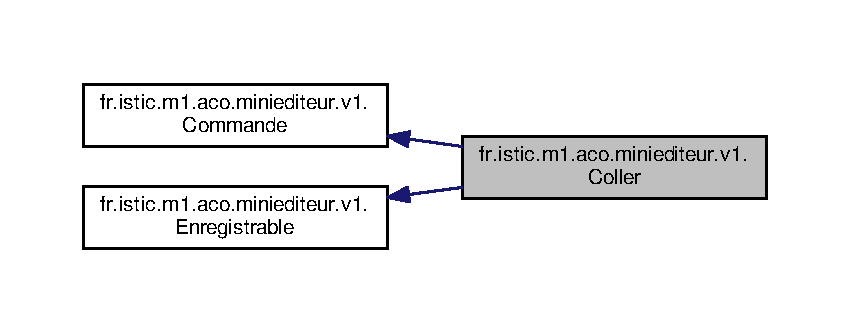
\includegraphics[width=350pt]{classfr_1_1istic_1_1m1_1_1aco_1_1miniediteur_1_1v1_1_1Coller__inherit__graph}
\end{center}
\end{figure}


Graphe de collaboration de fr.\+istic.\+m1.\+aco.\+miniediteur.\+v1.\+Coller\+:
\nopagebreak
\begin{figure}[H]
\begin{center}
\leavevmode
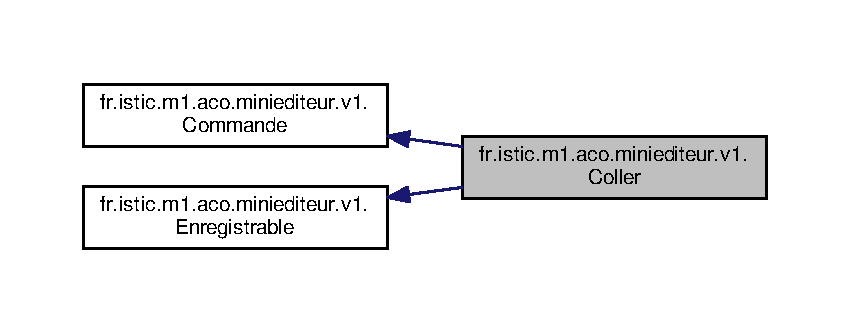
\includegraphics[width=350pt]{classfr_1_1istic_1_1m1_1_1aco_1_1miniediteur_1_1v1_1_1Coller__coll__graph}
\end{center}
\end{figure}
\subsection*{Fonctions membres publiques}
\begin{DoxyCompactItemize}
\item 
void \hyperlink{classfr_1_1istic_1_1m1_1_1aco_1_1miniediteur_1_1v1_1_1Coller_a753fef9385eac2cc41d99bf19bd486fe}{execute} ()
\begin{DoxyCompactList}\small\item\em Implémentation permettant d\textquotesingle{}effectuer l\textquotesingle{}action coller du \char`\"{}copié-\/collé\char`\"{}. \end{DoxyCompactList}\item 
\hyperlink{interfacefr_1_1istic_1_1m1_1_1aco_1_1miniediteur_1_1v1_1_1Memento}{Memento} \hyperlink{classfr_1_1istic_1_1m1_1_1aco_1_1miniediteur_1_1v1_1_1Coller_a7ec61b1f6fcc322d4a3548e4e1461689}{get\+Memento} ()
\begin{DoxyCompactList}\small\item\em Implémentation vierge de la méthode get\+Memento car l\textquotesingle{}action \hyperlink{classfr_1_1istic_1_1m1_1_1aco_1_1miniediteur_1_1v1_1_1Coller}{Coller} n\textquotesingle{}a pas de sauvegarde du texte à copier. \end{DoxyCompactList}\item 
\mbox{\Hypertarget{classfr_1_1istic_1_1m1_1_1aco_1_1miniediteur_1_1v1_1_1Coller_ae124aa0dd82f636e21afa91b01838edc}\label{classfr_1_1istic_1_1m1_1_1aco_1_1miniediteur_1_1v1_1_1Coller_ae124aa0dd82f636e21afa91b01838edc}} 
void \hyperlink{classfr_1_1istic_1_1m1_1_1aco_1_1miniediteur_1_1v1_1_1Coller_ae124aa0dd82f636e21afa91b01838edc}{set\+Memento} (\hyperlink{interfacefr_1_1istic_1_1m1_1_1aco_1_1miniediteur_1_1v1_1_1Memento}{Memento} m)
\begin{DoxyCompactList}\small\item\em Implémentation vierge de la méthode set\+Memento car l\textquotesingle{}action \hyperlink{classfr_1_1istic_1_1m1_1_1aco_1_1miniediteur_1_1v1_1_1Coller}{Coller} n\textquotesingle{}a pas de sauvegarde du texte à copier. \end{DoxyCompactList}\end{DoxyCompactItemize}


\subsection{Description détaillée}
Classe contrôlant le fonctionnement de la fonctionnalité permettant de \hyperlink{classfr_1_1istic_1_1m1_1_1aco_1_1miniediteur_1_1v1_1_1Coller}{Coller} dans un \char`\"{}copié-\/collé\char`\"{}. 

\subsection{Documentation des fonctions membres}
\mbox{\Hypertarget{classfr_1_1istic_1_1m1_1_1aco_1_1miniediteur_1_1v1_1_1Coller_a753fef9385eac2cc41d99bf19bd486fe}\label{classfr_1_1istic_1_1m1_1_1aco_1_1miniediteur_1_1v1_1_1Coller_a753fef9385eac2cc41d99bf19bd486fe}} 
\index{fr\+::istic\+::m1\+::aco\+::miniediteur\+::v1\+::\+Coller@{fr\+::istic\+::m1\+::aco\+::miniediteur\+::v1\+::\+Coller}!execute@{execute}}
\index{execute@{execute}!fr\+::istic\+::m1\+::aco\+::miniediteur\+::v1\+::\+Coller@{fr\+::istic\+::m1\+::aco\+::miniediteur\+::v1\+::\+Coller}}
\subsubsection{\texorpdfstring{execute()}{execute()}}
{\footnotesize\ttfamily void fr.\+istic.\+m1.\+aco.\+miniediteur.\+v1.\+Coller.\+execute (\begin{DoxyParamCaption}{ }\end{DoxyParamCaption})}



Implémentation permettant d\textquotesingle{}effectuer l\textquotesingle{}action coller du \char`\"{}copié-\/collé\char`\"{}. 

Action enregistrable et donc pouvant faire l\textquotesingle{}objet d\textquotesingle{}un défaire refaire. Fait appel à l\textquotesingle{}implémentation de la dite action du moteur. Est donc \char`\"{}implementation-\/dependent\char`\"{} du moteur. 

Implémente \hyperlink{interfacefr_1_1istic_1_1m1_1_1aco_1_1miniediteur_1_1v1_1_1Commande_a87a8a55bac4e81e32339248f79f7de4f}{fr.\+istic.\+m1.\+aco.\+miniediteur.\+v1.\+Commande}.

\mbox{\Hypertarget{classfr_1_1istic_1_1m1_1_1aco_1_1miniediteur_1_1v1_1_1Coller_a7ec61b1f6fcc322d4a3548e4e1461689}\label{classfr_1_1istic_1_1m1_1_1aco_1_1miniediteur_1_1v1_1_1Coller_a7ec61b1f6fcc322d4a3548e4e1461689}} 
\index{fr\+::istic\+::m1\+::aco\+::miniediteur\+::v1\+::\+Coller@{fr\+::istic\+::m1\+::aco\+::miniediteur\+::v1\+::\+Coller}!get\+Memento@{get\+Memento}}
\index{get\+Memento@{get\+Memento}!fr\+::istic\+::m1\+::aco\+::miniediteur\+::v1\+::\+Coller@{fr\+::istic\+::m1\+::aco\+::miniediteur\+::v1\+::\+Coller}}
\subsubsection{\texorpdfstring{get\+Memento()}{getMemento()}}
{\footnotesize\ttfamily \hyperlink{interfacefr_1_1istic_1_1m1_1_1aco_1_1miniediteur_1_1v1_1_1Memento}{Memento} fr.\+istic.\+m1.\+aco.\+miniediteur.\+v1.\+Coller.\+get\+Memento (\begin{DoxyParamCaption}{ }\end{DoxyParamCaption})}



Implémentation vierge de la méthode get\+Memento car l\textquotesingle{}action \hyperlink{classfr_1_1istic_1_1m1_1_1aco_1_1miniediteur_1_1v1_1_1Coller}{Coller} n\textquotesingle{}a pas de sauvegarde du texte à copier. 

\begin{DoxyNote}{Note}
N\textquotesingle{}ayant pas de sauvegarde du texte à copier pour réutiliser \hyperlink{classfr_1_1istic_1_1m1_1_1aco_1_1miniediteur_1_1v1_1_1Coller}{Coller} dans une action \hyperlink{classfr_1_1istic_1_1m1_1_1aco_1_1miniediteur_1_1v1_1_1Refaire}{Refaire} il faut au préalable avoir enregistré soit \hyperlink{classfr_1_1istic_1_1m1_1_1aco_1_1miniediteur_1_1v1_1_1Copier}{Copier} soit \hyperlink{classfr_1_1istic_1_1m1_1_1aco_1_1miniediteur_1_1v1_1_1Couper}{Couper}. 
\end{DoxyNote}
\begin{DoxyReturn}{Renvoie}
Un null comme \hyperlink{classfr_1_1istic_1_1m1_1_1aco_1_1miniediteur_1_1v1_1_1Coller}{Coller} n\textquotesingle{}a pas de sauvegarde 
\end{DoxyReturn}


Implémente \hyperlink{interfacefr_1_1istic_1_1m1_1_1aco_1_1miniediteur_1_1v1_1_1Enregistrable}{fr.\+istic.\+m1.\+aco.\+miniediteur.\+v1.\+Enregistrable}.



La documentation de cette classe a été générée à partir du fichier suivant \+:\begin{DoxyCompactItemize}
\item 
src/fr/istic/m1/aco/miniediteur/v1/\hyperlink{Coller_8java}{Coller.\+java}\end{DoxyCompactItemize}

\hypertarget{interfacefr_1_1istic_1_1m1_1_1aco_1_1miniediteur_1_1v1_1_1Commande}{}\section{Référence de l\textquotesingle{}interface fr.\+istic.\+m1.\+aco.\+miniediteur.\+v1.\+Commande}
\label{interfacefr_1_1istic_1_1m1_1_1aco_1_1miniediteur_1_1v1_1_1Commande}\index{fr.\+istic.\+m1.\+aco.\+miniediteur.\+v1.\+Commande@{fr.\+istic.\+m1.\+aco.\+miniediteur.\+v1.\+Commande}}


Interface décrivant une commande déclenchée par une action sur l\textquotesingle{}\hyperlink{interfacefr_1_1istic_1_1m1_1_1aco_1_1miniediteur_1_1v1_1_1IHM}{I\+HM} de l\textquotesingle{}Utilisateur.  




Graphe d\textquotesingle{}héritage de fr.\+istic.\+m1.\+aco.\+miniediteur.\+v1.\+Commande\+:
\nopagebreak
\begin{figure}[H]
\begin{center}
\leavevmode
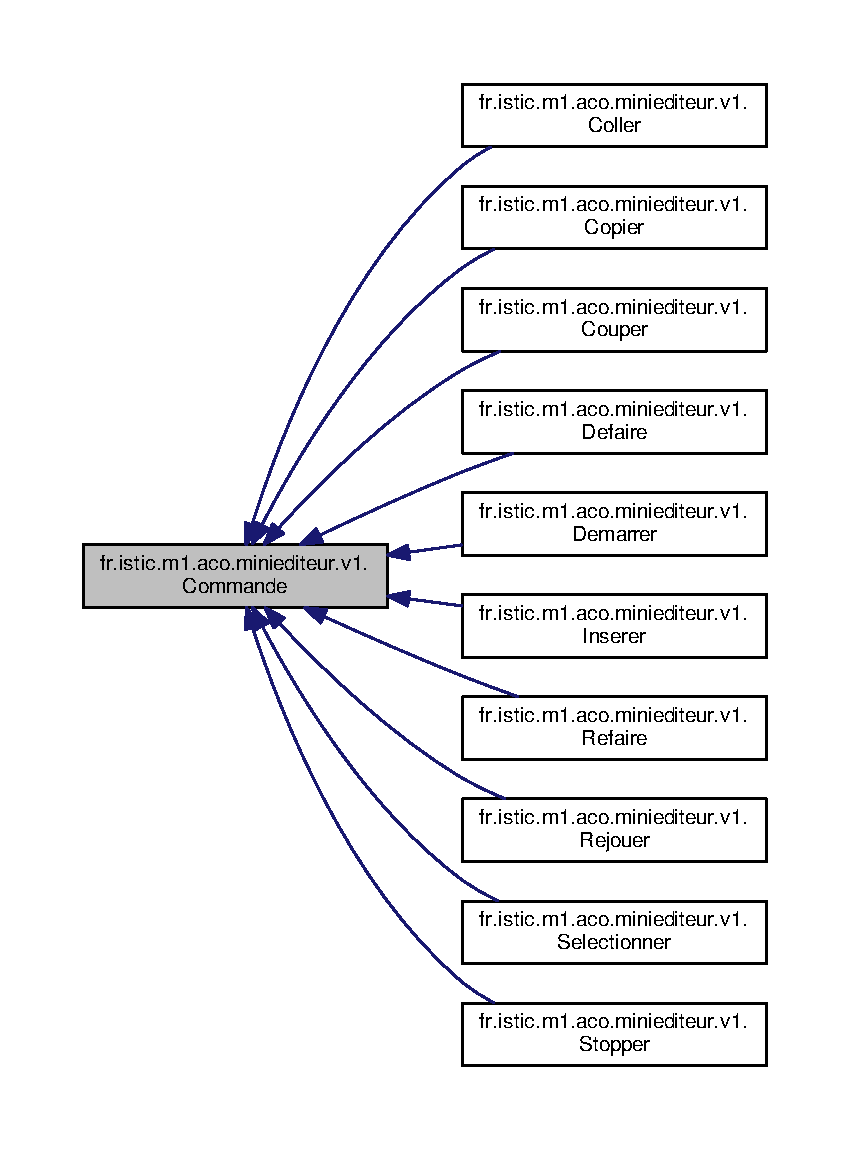
\includegraphics[width=350pt]{interfacefr_1_1istic_1_1m1_1_1aco_1_1miniediteur_1_1v1_1_1Commande__inherit__graph}
\end{center}
\end{figure}
\subsection*{Fonctions membres publiques}
\begin{DoxyCompactItemize}
\item 
\mbox{\Hypertarget{interfacefr_1_1istic_1_1m1_1_1aco_1_1miniediteur_1_1v1_1_1Commande_a87a8a55bac4e81e32339248f79f7de4f}\label{interfacefr_1_1istic_1_1m1_1_1aco_1_1miniediteur_1_1v1_1_1Commande_a87a8a55bac4e81e32339248f79f7de4f}} 
void \hyperlink{interfacefr_1_1istic_1_1m1_1_1aco_1_1miniediteur_1_1v1_1_1Commande_a87a8a55bac4e81e32339248f79f7de4f}{execute} ()
\begin{DoxyCompactList}\small\item\em Méthode commune aux commandes devant implémenter leur action quand déclenchée par l\textquotesingle{}\hyperlink{interfacefr_1_1istic_1_1m1_1_1aco_1_1miniediteur_1_1v1_1_1IHM}{I\+HM}. \end{DoxyCompactList}\end{DoxyCompactItemize}


\subsection{Description détaillée}
Interface décrivant une commande déclenchée par une action sur l\textquotesingle{}\hyperlink{interfacefr_1_1istic_1_1m1_1_1aco_1_1miniediteur_1_1v1_1_1IHM}{I\+HM} de l\textquotesingle{}Utilisateur. 

Élément d\textquotesingle{}intégration d\textquotesingle{}un design pattern \char`\"{}\+Command\char`\"{} remplissant le rôle \char`\"{}command\char`\"{} 

La documentation de cette interface a été générée à partir du fichier suivant \+:\begin{DoxyCompactItemize}
\item 
src/fr/istic/m1/aco/miniediteur/v1/\hyperlink{Commande_8java}{Commande.\+java}\end{DoxyCompactItemize}

\hypertarget{classfr_1_1istic_1_1m1_1_1aco_1_1miniediteur_1_1v1_1_1Copier}{}\section{Référence de la classe fr.\+istic.\+m1.\+aco.\+miniediteur.\+v1.\+Copier}
\label{classfr_1_1istic_1_1m1_1_1aco_1_1miniediteur_1_1v1_1_1Copier}\index{fr.\+istic.\+m1.\+aco.\+miniediteur.\+v1.\+Copier@{fr.\+istic.\+m1.\+aco.\+miniediteur.\+v1.\+Copier}}


Classe contrôlant le fonctionnement de la fonctionnalité permettant de \hyperlink{classfr_1_1istic_1_1m1_1_1aco_1_1miniediteur_1_1v1_1_1Copier}{Copier} dans un \char`\"{}copié-\/collé\char`\"{}.  




Graphe d\textquotesingle{}héritage de fr.\+istic.\+m1.\+aco.\+miniediteur.\+v1.\+Copier\+:
\nopagebreak
\begin{figure}[H]
\begin{center}
\leavevmode
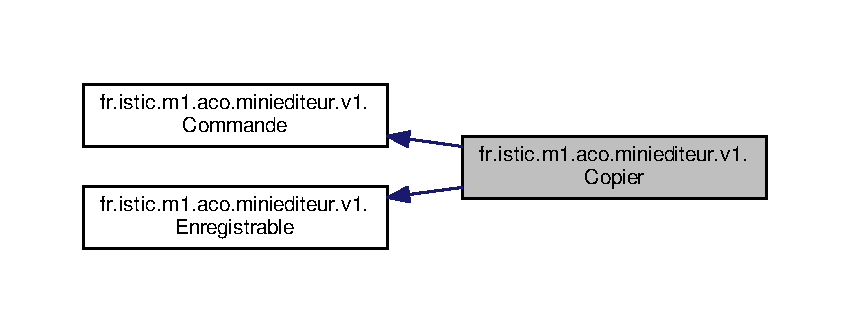
\includegraphics[width=350pt]{classfr_1_1istic_1_1m1_1_1aco_1_1miniediteur_1_1v1_1_1Copier__inherit__graph}
\end{center}
\end{figure}


Graphe de collaboration de fr.\+istic.\+m1.\+aco.\+miniediteur.\+v1.\+Copier\+:
\nopagebreak
\begin{figure}[H]
\begin{center}
\leavevmode
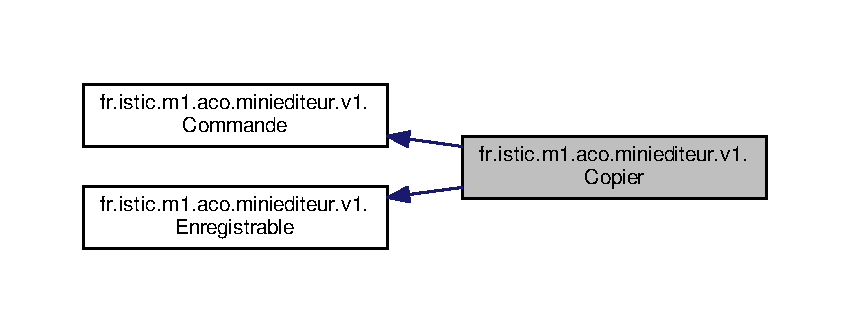
\includegraphics[width=350pt]{classfr_1_1istic_1_1m1_1_1aco_1_1miniediteur_1_1v1_1_1Copier__coll__graph}
\end{center}
\end{figure}
\subsection*{Fonctions membres publiques}
\begin{DoxyCompactItemize}
\item 
void \hyperlink{classfr_1_1istic_1_1m1_1_1aco_1_1miniediteur_1_1v1_1_1Copier_ac0a36f63af9a9c11bdc4c043923ded58}{execute} ()
\begin{DoxyCompactList}\small\item\em Implémentation permettant d\textquotesingle{}effectuer l\textquotesingle{}action copier du \char`\"{}copié-\/collé\char`\"{}. \end{DoxyCompactList}\item 
\hyperlink{interfacefr_1_1istic_1_1m1_1_1aco_1_1miniediteur_1_1v1_1_1Memento}{Memento} \hyperlink{classfr_1_1istic_1_1m1_1_1aco_1_1miniediteur_1_1v1_1_1Copier_af7810fb486b49fcf6ca28958de33c7d0}{get\+Memento} ()
\begin{DoxyCompactList}\small\item\em Implémentation vierge de la méthode get\+Memento car l\textquotesingle{}action \hyperlink{classfr_1_1istic_1_1m1_1_1aco_1_1miniediteur_1_1v1_1_1Copier}{Copier} n\textquotesingle{}a pas de sauvegarde du texte à copier. \end{DoxyCompactList}\item 
\mbox{\Hypertarget{classfr_1_1istic_1_1m1_1_1aco_1_1miniediteur_1_1v1_1_1Copier_a4e1de8f07ded1ed4e33d8c8e6385a0a6}\label{classfr_1_1istic_1_1m1_1_1aco_1_1miniediteur_1_1v1_1_1Copier_a4e1de8f07ded1ed4e33d8c8e6385a0a6}} 
void \hyperlink{classfr_1_1istic_1_1m1_1_1aco_1_1miniediteur_1_1v1_1_1Copier_a4e1de8f07ded1ed4e33d8c8e6385a0a6}{set\+Memento} (\hyperlink{interfacefr_1_1istic_1_1m1_1_1aco_1_1miniediteur_1_1v1_1_1Memento}{Memento} m)
\begin{DoxyCompactList}\small\item\em Implémentation vierge de la méthode set\+Memento car l\textquotesingle{}action \hyperlink{classfr_1_1istic_1_1m1_1_1aco_1_1miniediteur_1_1v1_1_1Copier}{Copier} n\textquotesingle{}a pas de sauvegarde du texte à copier. \end{DoxyCompactList}\end{DoxyCompactItemize}


\subsection{Description détaillée}
Classe contrôlant le fonctionnement de la fonctionnalité permettant de \hyperlink{classfr_1_1istic_1_1m1_1_1aco_1_1miniediteur_1_1v1_1_1Copier}{Copier} dans un \char`\"{}copié-\/collé\char`\"{}. 

\subsection{Documentation des fonctions membres}
\mbox{\Hypertarget{classfr_1_1istic_1_1m1_1_1aco_1_1miniediteur_1_1v1_1_1Copier_ac0a36f63af9a9c11bdc4c043923ded58}\label{classfr_1_1istic_1_1m1_1_1aco_1_1miniediteur_1_1v1_1_1Copier_ac0a36f63af9a9c11bdc4c043923ded58}} 
\index{fr\+::istic\+::m1\+::aco\+::miniediteur\+::v1\+::\+Copier@{fr\+::istic\+::m1\+::aco\+::miniediteur\+::v1\+::\+Copier}!execute@{execute}}
\index{execute@{execute}!fr\+::istic\+::m1\+::aco\+::miniediteur\+::v1\+::\+Copier@{fr\+::istic\+::m1\+::aco\+::miniediteur\+::v1\+::\+Copier}}
\subsubsection{\texorpdfstring{execute()}{execute()}}
{\footnotesize\ttfamily void fr.\+istic.\+m1.\+aco.\+miniediteur.\+v1.\+Copier.\+execute (\begin{DoxyParamCaption}{ }\end{DoxyParamCaption})}



Implémentation permettant d\textquotesingle{}effectuer l\textquotesingle{}action copier du \char`\"{}copié-\/collé\char`\"{}. 

Action enregistrable et donc pouvant faire l\textquotesingle{}objet d\textquotesingle{}un défaire refaire. Fait appel à l\textquotesingle{}implémentation de la dite action du moteur. Est donc \char`\"{}implementation-\/dependent\char`\"{} du moteur. 

Implémente \hyperlink{interfacefr_1_1istic_1_1m1_1_1aco_1_1miniediteur_1_1v1_1_1Commande_a87a8a55bac4e81e32339248f79f7de4f}{fr.\+istic.\+m1.\+aco.\+miniediteur.\+v1.\+Commande}.

\mbox{\Hypertarget{classfr_1_1istic_1_1m1_1_1aco_1_1miniediteur_1_1v1_1_1Copier_af7810fb486b49fcf6ca28958de33c7d0}\label{classfr_1_1istic_1_1m1_1_1aco_1_1miniediteur_1_1v1_1_1Copier_af7810fb486b49fcf6ca28958de33c7d0}} 
\index{fr\+::istic\+::m1\+::aco\+::miniediteur\+::v1\+::\+Copier@{fr\+::istic\+::m1\+::aco\+::miniediteur\+::v1\+::\+Copier}!get\+Memento@{get\+Memento}}
\index{get\+Memento@{get\+Memento}!fr\+::istic\+::m1\+::aco\+::miniediteur\+::v1\+::\+Copier@{fr\+::istic\+::m1\+::aco\+::miniediteur\+::v1\+::\+Copier}}
\subsubsection{\texorpdfstring{get\+Memento()}{getMemento()}}
{\footnotesize\ttfamily \hyperlink{interfacefr_1_1istic_1_1m1_1_1aco_1_1miniediteur_1_1v1_1_1Memento}{Memento} fr.\+istic.\+m1.\+aco.\+miniediteur.\+v1.\+Copier.\+get\+Memento (\begin{DoxyParamCaption}{ }\end{DoxyParamCaption})}



Implémentation vierge de la méthode get\+Memento car l\textquotesingle{}action \hyperlink{classfr_1_1istic_1_1m1_1_1aco_1_1miniediteur_1_1v1_1_1Copier}{Copier} n\textquotesingle{}a pas de sauvegarde du texte à copier. 

\begin{DoxyNote}{Note}
N\textquotesingle{}ayant pas de sauvegarde du texte à copier pour réutiliser \hyperlink{classfr_1_1istic_1_1m1_1_1aco_1_1miniediteur_1_1v1_1_1Copier}{Copier} dans une action \hyperlink{classfr_1_1istic_1_1m1_1_1aco_1_1miniediteur_1_1v1_1_1Refaire}{Refaire} avec l\textquotesingle{}intention de remettre texte précis il faut avoir au préalable enregistrer \hyperlink{classfr_1_1istic_1_1m1_1_1aco_1_1miniediteur_1_1v1_1_1Selectionner}{Selectionner} aussi. 
\end{DoxyNote}
\begin{DoxyReturn}{Renvoie}
Un null comme \hyperlink{classfr_1_1istic_1_1m1_1_1aco_1_1miniediteur_1_1v1_1_1Copier}{Copier} n\textquotesingle{}a pas de sauvegarde 
\end{DoxyReturn}


Implémente \hyperlink{interfacefr_1_1istic_1_1m1_1_1aco_1_1miniediteur_1_1v1_1_1Enregistrable_aadf173c765d103d3924bbb688c45abb6}{fr.\+istic.\+m1.\+aco.\+miniediteur.\+v1.\+Enregistrable}.



La documentation de cette classe a été générée à partir du fichier suivant \+:\begin{DoxyCompactItemize}
\item 
src/fr/istic/m1/aco/miniediteur/v1/\hyperlink{Copier_8java}{Copier.\+java}\end{DoxyCompactItemize}

\hypertarget{classfr_1_1istic_1_1m1_1_1aco_1_1miniediteur_1_1v1_1_1Couper}{}\section{Référence de la classe fr.\+istic.\+m1.\+aco.\+miniediteur.\+v1.\+Couper}
\label{classfr_1_1istic_1_1m1_1_1aco_1_1miniediteur_1_1v1_1_1Couper}\index{fr.\+istic.\+m1.\+aco.\+miniediteur.\+v1.\+Couper@{fr.\+istic.\+m1.\+aco.\+miniediteur.\+v1.\+Couper}}


Graphe d\textquotesingle{}héritage de fr.\+istic.\+m1.\+aco.\+miniediteur.\+v1.\+Couper\+:
\nopagebreak
\begin{figure}[H]
\begin{center}
\leavevmode
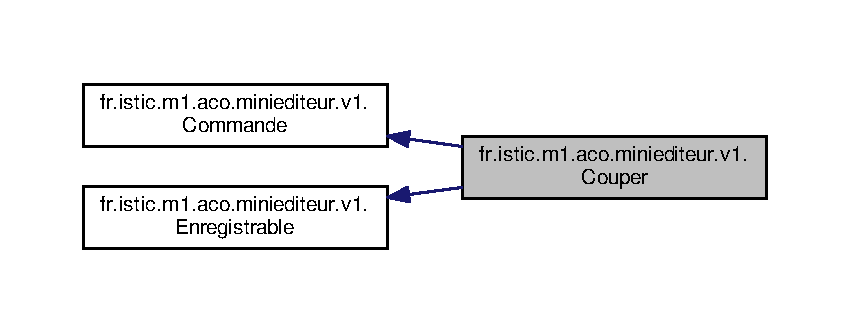
\includegraphics[width=350pt]{classfr_1_1istic_1_1m1_1_1aco_1_1miniediteur_1_1v1_1_1Couper__inherit__graph}
\end{center}
\end{figure}


Graphe de collaboration de fr.\+istic.\+m1.\+aco.\+miniediteur.\+v1.\+Couper\+:
\nopagebreak
\begin{figure}[H]
\begin{center}
\leavevmode
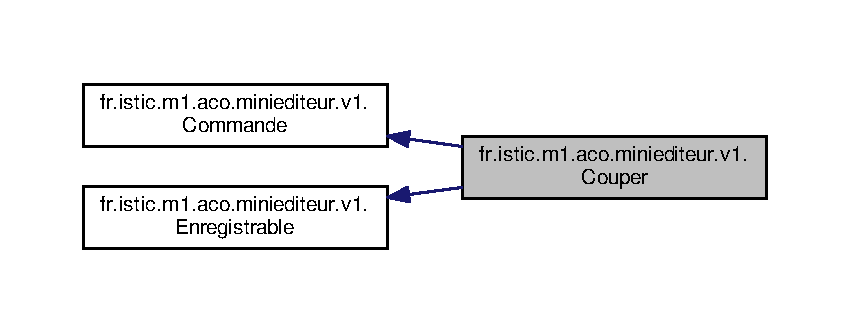
\includegraphics[width=350pt]{classfr_1_1istic_1_1m1_1_1aco_1_1miniediteur_1_1v1_1_1Couper__coll__graph}
\end{center}
\end{figure}
\subsection*{Fonctions membres publiques}
\begin{DoxyCompactItemize}
\item 
\mbox{\Hypertarget{classfr_1_1istic_1_1m1_1_1aco_1_1miniediteur_1_1v1_1_1Couper_aa646ea059793eb7db2066175369cbdae}\label{classfr_1_1istic_1_1m1_1_1aco_1_1miniediteur_1_1v1_1_1Couper_aa646ea059793eb7db2066175369cbdae}} 
void \hyperlink{classfr_1_1istic_1_1m1_1_1aco_1_1miniediteur_1_1v1_1_1Couper_aa646ea059793eb7db2066175369cbdae}{execute} ()
\begin{DoxyCompactList}\small\item\em Méthode commune aux commandes devant implémenter leur action quand déclenchée par l\textquotesingle{}\hyperlink{interfacefr_1_1istic_1_1m1_1_1aco_1_1miniediteur_1_1v1_1_1IHM}{I\+HM}. \end{DoxyCompactList}\item 
\mbox{\Hypertarget{classfr_1_1istic_1_1m1_1_1aco_1_1miniediteur_1_1v1_1_1Couper_aa4f63cd2eb49ae3b96f175989d93c338}\label{classfr_1_1istic_1_1m1_1_1aco_1_1miniediteur_1_1v1_1_1Couper_aa4f63cd2eb49ae3b96f175989d93c338}} 
\hyperlink{interfacefr_1_1istic_1_1m1_1_1aco_1_1miniediteur_1_1v1_1_1Memento}{Memento} {\bfseries get\+Memento} ()
\item 
\mbox{\Hypertarget{classfr_1_1istic_1_1m1_1_1aco_1_1miniediteur_1_1v1_1_1Couper_a36f0578188f4526c624565c9afa4abc8}\label{classfr_1_1istic_1_1m1_1_1aco_1_1miniediteur_1_1v1_1_1Couper_a36f0578188f4526c624565c9afa4abc8}} 
void {\bfseries set\+Memento} (\hyperlink{interfacefr_1_1istic_1_1m1_1_1aco_1_1miniediteur_1_1v1_1_1Memento}{Memento} m)
\end{DoxyCompactItemize}


La documentation de cette classe a été générée à partir du fichier suivant \+:\begin{DoxyCompactItemize}
\item 
src/fr/istic/m1/aco/miniediteur/v1/Couper.\+java\end{DoxyCompactItemize}

\hypertarget{classfr_1_1istic_1_1m1_1_1aco_1_1miniediteur_1_1v1_1_1Defaire}{}\section{Référence de la classe fr.\+istic.\+m1.\+aco.\+miniediteur.\+v1.\+Defaire}
\label{classfr_1_1istic_1_1m1_1_1aco_1_1miniediteur_1_1v1_1_1Defaire}\index{fr.\+istic.\+m1.\+aco.\+miniediteur.\+v1.\+Defaire@{fr.\+istic.\+m1.\+aco.\+miniediteur.\+v1.\+Defaire}}


Classe contrôlant le fonctionnement de la fonctionnalité permettant de Défaire dans un \char`\"{}défaire-\/refaire\char`\"{}.  




Graphe d\textquotesingle{}héritage de fr.\+istic.\+m1.\+aco.\+miniediteur.\+v1.\+Defaire\+:\nopagebreak
\begin{figure}[H]
\begin{center}
\leavevmode
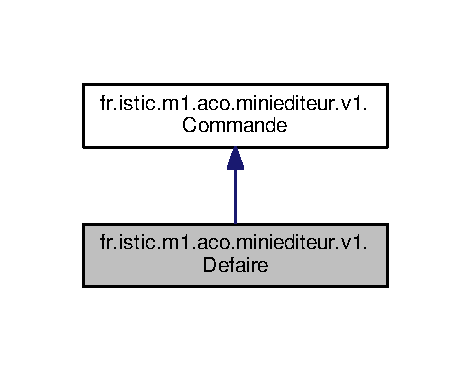
\includegraphics[width=226pt]{classfr_1_1istic_1_1m1_1_1aco_1_1miniediteur_1_1v1_1_1Defaire__inherit__graph}
\end{center}
\end{figure}


Graphe de collaboration de fr.\+istic.\+m1.\+aco.\+miniediteur.\+v1.\+Defaire\+:\nopagebreak
\begin{figure}[H]
\begin{center}
\leavevmode
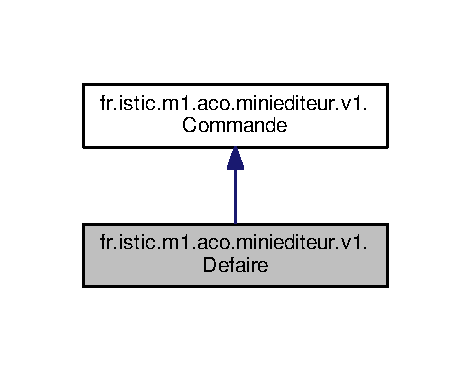
\includegraphics[width=226pt]{classfr_1_1istic_1_1m1_1_1aco_1_1miniediteur_1_1v1_1_1Defaire__coll__graph}
\end{center}
\end{figure}
\subsection*{Fonctions membres publiques}
\begin{DoxyCompactItemize}
\item 
void \hyperlink{classfr_1_1istic_1_1m1_1_1aco_1_1miniediteur_1_1v1_1_1Defaire_a3b8c0beab28336ae060284fdf4a78a52}{execute} ()
\begin{DoxyCompactList}\small\item\em Implémentation permettant d\textquotesingle{}effectuer l\textquotesingle{}action défaire du \char`\"{}défaire-\/refaire\char`\"{}. \end{DoxyCompactList}\end{DoxyCompactItemize}


\subsection{Description détaillée}
Classe contrôlant le fonctionnement de la fonctionnalité permettant de Défaire dans un \char`\"{}défaire-\/refaire\char`\"{}. 

\begin{DoxyNote}{Note}
Dans la spécification de la version 3 du Mini-\/Éditeur cette commande a été introduite et elle ne doit pas obligatoirement être enregistrée. La fonctionnalité d\textquotesingle{}enregistrement n\textquotesingle{}est donc pas implémentée. 
\end{DoxyNote}


\subsection{Documentation des fonctions membres}
\mbox{\Hypertarget{classfr_1_1istic_1_1m1_1_1aco_1_1miniediteur_1_1v1_1_1Defaire_a3b8c0beab28336ae060284fdf4a78a52}\label{classfr_1_1istic_1_1m1_1_1aco_1_1miniediteur_1_1v1_1_1Defaire_a3b8c0beab28336ae060284fdf4a78a52}} 
\index{fr\+::istic\+::m1\+::aco\+::miniediteur\+::v1\+::\+Defaire@{fr\+::istic\+::m1\+::aco\+::miniediteur\+::v1\+::\+Defaire}!execute@{execute}}
\index{execute@{execute}!fr\+::istic\+::m1\+::aco\+::miniediteur\+::v1\+::\+Defaire@{fr\+::istic\+::m1\+::aco\+::miniediteur\+::v1\+::\+Defaire}}
\subsubsection{\texorpdfstring{execute()}{execute()}}
{\footnotesize\ttfamily void fr.\+istic.\+m1.\+aco.\+miniediteur.\+v1.\+Defaire.\+execute (\begin{DoxyParamCaption}{ }\end{DoxyParamCaption})}



Implémentation permettant d\textquotesingle{}effectuer l\textquotesingle{}action défaire du \char`\"{}défaire-\/refaire\char`\"{}. 

Fait appel à l\textquotesingle{}implémentation de la dite action du \hyperlink{interfacefr_1_1istic_1_1m1_1_1aco_1_1miniediteur_1_1v1_1_1GestionnaireDefaireRefaire}{Gestionnaire\+Defaire\+Refaire}. Est donc \char`\"{}implementation-\/dependent\char`\"{} du \hyperlink{interfacefr_1_1istic_1_1m1_1_1aco_1_1miniediteur_1_1v1_1_1GestionnaireDefaireRefaire}{Gestionnaire\+Defaire\+Refaire}. 

Implémente \hyperlink{interfacefr_1_1istic_1_1m1_1_1aco_1_1miniediteur_1_1v1_1_1Commande_a87a8a55bac4e81e32339248f79f7de4f}{fr.\+istic.\+m1.\+aco.\+miniediteur.\+v1.\+Commande}.



La documentation de cette classe a été générée à partir du fichier suivant \+:\begin{DoxyCompactItemize}
\item 
src/fr/istic/m1/aco/miniediteur/v1/\hyperlink{Defaire_8java}{Defaire.\+java}\end{DoxyCompactItemize}

\hypertarget{classfr_1_1istic_1_1m1_1_1aco_1_1miniediteur_1_1v1_1_1Demarrer}{}\section{Référence de la classe fr.\+istic.\+m1.\+aco.\+miniediteur.\+v1.\+Demarrer}
\label{classfr_1_1istic_1_1m1_1_1aco_1_1miniediteur_1_1v1_1_1Demarrer}\index{fr.\+istic.\+m1.\+aco.\+miniediteur.\+v1.\+Demarrer@{fr.\+istic.\+m1.\+aco.\+miniediteur.\+v1.\+Demarrer}}


Classe contrôlant le fonctionnement de la fonctionnalité permettant de débuter l\textquotesingle{}enregistrement d\textquotesingle{}une macro.  




Graphe d\textquotesingle{}héritage de fr.\+istic.\+m1.\+aco.\+miniediteur.\+v1.\+Demarrer\+:\nopagebreak
\begin{figure}[H]
\begin{center}
\leavevmode
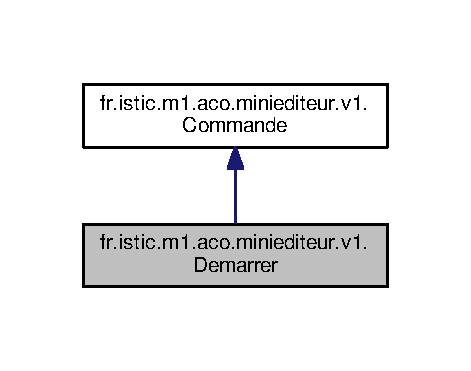
\includegraphics[width=226pt]{classfr_1_1istic_1_1m1_1_1aco_1_1miniediteur_1_1v1_1_1Demarrer__inherit__graph}
\end{center}
\end{figure}


Graphe de collaboration de fr.\+istic.\+m1.\+aco.\+miniediteur.\+v1.\+Demarrer\+:\nopagebreak
\begin{figure}[H]
\begin{center}
\leavevmode
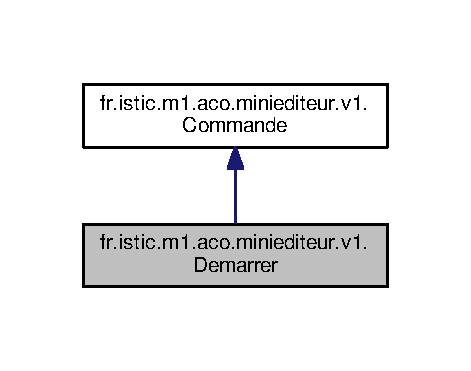
\includegraphics[width=226pt]{classfr_1_1istic_1_1m1_1_1aco_1_1miniediteur_1_1v1_1_1Demarrer__coll__graph}
\end{center}
\end{figure}
\subsection*{Fonctions membres publiques}
\begin{DoxyCompactItemize}
\item 
void \hyperlink{classfr_1_1istic_1_1m1_1_1aco_1_1miniediteur_1_1v1_1_1Demarrer_a1de3c107a8ee460c70a5b98e6b7edd69}{execute} ()
\begin{DoxyCompactList}\small\item\em Implémentation permettant d\textquotesingle{}effectuer l\textquotesingle{}action débutant l\textquotesingle{}enregistrement d\textquotesingle{}une macro. \end{DoxyCompactList}\end{DoxyCompactItemize}


\subsection{Description détaillée}
Classe contrôlant le fonctionnement de la fonctionnalité permettant de débuter l\textquotesingle{}enregistrement d\textquotesingle{}une macro. 

Fonctionnalité introduite dans la spécification de la version 2 du Mini-\/Éditeur. N\textquotesingle{}est pas elle même enregistrable conformément à la spécification pour éviter un empilement d\textquotesingle{}enregistrements qui résulterait en un écrasement des précédents. 

\subsection{Documentation des fonctions membres}
\mbox{\Hypertarget{classfr_1_1istic_1_1m1_1_1aco_1_1miniediteur_1_1v1_1_1Demarrer_a1de3c107a8ee460c70a5b98e6b7edd69}\label{classfr_1_1istic_1_1m1_1_1aco_1_1miniediteur_1_1v1_1_1Demarrer_a1de3c107a8ee460c70a5b98e6b7edd69}} 
\index{fr\+::istic\+::m1\+::aco\+::miniediteur\+::v1\+::\+Demarrer@{fr\+::istic\+::m1\+::aco\+::miniediteur\+::v1\+::\+Demarrer}!execute@{execute}}
\index{execute@{execute}!fr\+::istic\+::m1\+::aco\+::miniediteur\+::v1\+::\+Demarrer@{fr\+::istic\+::m1\+::aco\+::miniediteur\+::v1\+::\+Demarrer}}
\subsubsection{\texorpdfstring{execute()}{execute()}}
{\footnotesize\ttfamily void fr.\+istic.\+m1.\+aco.\+miniediteur.\+v1.\+Demarrer.\+execute (\begin{DoxyParamCaption}{ }\end{DoxyParamCaption})}



Implémentation permettant d\textquotesingle{}effectuer l\textquotesingle{}action débutant l\textquotesingle{}enregistrement d\textquotesingle{}une macro. 

Fait appel à l\textquotesingle{}implémentation de l\textquotesingle{}enregistremenent. Est donc \char`\"{}implementation-\/dependent\char`\"{} de l\textquotesingle{}\hyperlink{interfacefr_1_1istic_1_1m1_1_1aco_1_1miniediteur_1_1v1_1_1Enregistreur}{Enregistreur}. 

Implémente \hyperlink{interfacefr_1_1istic_1_1m1_1_1aco_1_1miniediteur_1_1v1_1_1Commande_a87a8a55bac4e81e32339248f79f7de4f}{fr.\+istic.\+m1.\+aco.\+miniediteur.\+v1.\+Commande}.



La documentation de cette classe a été générée à partir du fichier suivant \+:\begin{DoxyCompactItemize}
\item 
src/fr/istic/m1/aco/miniediteur/v1/\hyperlink{Demarrer_8java}{Demarrer.\+java}\end{DoxyCompactItemize}

\hypertarget{classfr_1_1istic_1_1m1_1_1aco_1_1miniediteur_1_1v1_1_1Editeur}{}\section{Référence de la classe fr.\+istic.\+m1.\+aco.\+miniediteur.\+v1.\+Editeur}
\label{classfr_1_1istic_1_1m1_1_1aco_1_1miniediteur_1_1v1_1_1Editeur}\index{fr.\+istic.\+m1.\+aco.\+miniediteur.\+v1.\+Editeur@{fr.\+istic.\+m1.\+aco.\+miniediteur.\+v1.\+Editeur}}


La documentation de cette classe a été générée à partir du fichier suivant \+:\begin{DoxyCompactItemize}
\item 
src/fr/istic/m1/aco/miniediteur/v1/Editeur.\+java\end{DoxyCompactItemize}

\hypertarget{interfacefr_1_1istic_1_1m1_1_1aco_1_1miniediteur_1_1v1_1_1Enregistrable}{}\section{Référence de l\textquotesingle{}interface fr.\+istic.\+m1.\+aco.\+miniediteur.\+v1.\+Enregistrable}
\label{interfacefr_1_1istic_1_1m1_1_1aco_1_1miniediteur_1_1v1_1_1Enregistrable}\index{fr.\+istic.\+m1.\+aco.\+miniediteur.\+v1.\+Enregistrable@{fr.\+istic.\+m1.\+aco.\+miniediteur.\+v1.\+Enregistrable}}


Interface décrivant des actions pouvant faire l\textquotesingle{}objet d\textquotesingle{}un enregistrement pour une macro.  




Graphe d\textquotesingle{}héritage de fr.\+istic.\+m1.\+aco.\+miniediteur.\+v1.\+Enregistrable\+:
\nopagebreak
\begin{figure}[H]
\begin{center}
\leavevmode
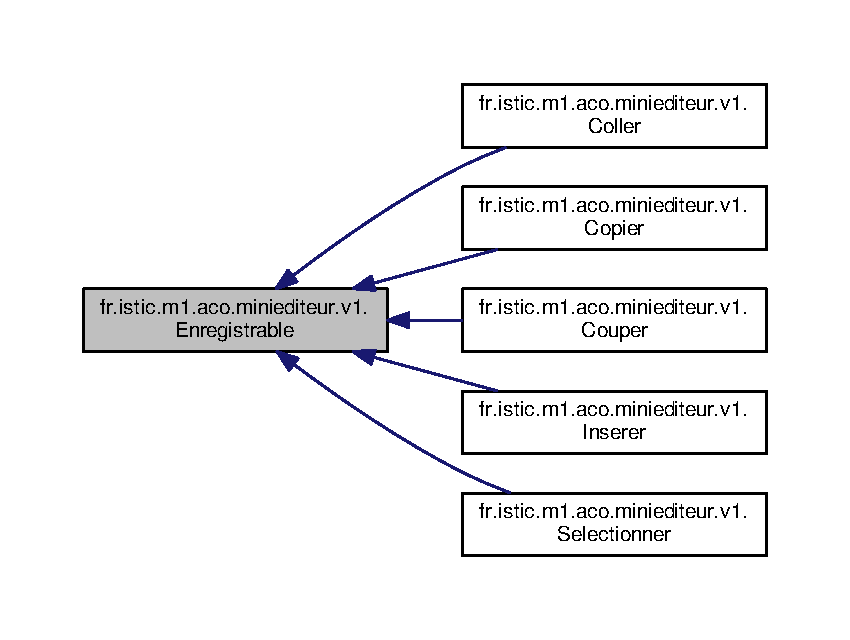
\includegraphics[width=350pt]{interfacefr_1_1istic_1_1m1_1_1aco_1_1miniediteur_1_1v1_1_1Enregistrable__inherit__graph}
\end{center}
\end{figure}
\subsection*{Fonctions membres publiques}
\begin{DoxyCompactItemize}
\item 
\hyperlink{interfacefr_1_1istic_1_1m1_1_1aco_1_1miniediteur_1_1v1_1_1Memento}{Memento} \hyperlink{interfacefr_1_1istic_1_1m1_1_1aco_1_1miniediteur_1_1v1_1_1Enregistrable_aadf173c765d103d3924bbb688c45abb6}{get\+Memento} ()
\begin{DoxyCompactList}\small\item\em Opération permettant d\textquotesingle{}obtenir une copie de l\textquotesingle{}état d\textquotesingle{}une opération requérant une sauvegarde pour pouvoir être refaire ultérieurement. \end{DoxyCompactList}\item 
void \hyperlink{interfacefr_1_1istic_1_1m1_1_1aco_1_1miniediteur_1_1v1_1_1Enregistrable_a949bb6784743800c2d743def265f41b1}{set\+Memento} (\hyperlink{interfacefr_1_1istic_1_1m1_1_1aco_1_1miniediteur_1_1v1_1_1Memento}{Memento} m)
\begin{DoxyCompactList}\small\item\em Opération permettant de réinitialiser la commande par rapport à un état précédent donné sous la forme d\textquotesingle{}un \hyperlink{interfacefr_1_1istic_1_1m1_1_1aco_1_1miniediteur_1_1v1_1_1Memento}{Memento}. \end{DoxyCompactList}\end{DoxyCompactItemize}


\subsection{Description détaillée}
Interface décrivant des actions pouvant faire l\textquotesingle{}objet d\textquotesingle{}un enregistrement pour une macro. 

Permet de séparer clairement les actions pouvant être enregistrée des autres et fourni des opérations nécéssaires à l\textquotesingle{}enregistrement. Rempli le rôle \char`\"{}originator\char`\"{} du design pattern \hyperlink{interfacefr_1_1istic_1_1m1_1_1aco_1_1miniediteur_1_1v1_1_1Memento}{Memento}. 

\subsection{Documentation des fonctions membres}
\mbox{\Hypertarget{interfacefr_1_1istic_1_1m1_1_1aco_1_1miniediteur_1_1v1_1_1Enregistrable_aadf173c765d103d3924bbb688c45abb6}\label{interfacefr_1_1istic_1_1m1_1_1aco_1_1miniediteur_1_1v1_1_1Enregistrable_aadf173c765d103d3924bbb688c45abb6}} 
\index{fr\+::istic\+::m1\+::aco\+::miniediteur\+::v1\+::\+Enregistrable@{fr\+::istic\+::m1\+::aco\+::miniediteur\+::v1\+::\+Enregistrable}!get\+Memento@{get\+Memento}}
\index{get\+Memento@{get\+Memento}!fr\+::istic\+::m1\+::aco\+::miniediteur\+::v1\+::\+Enregistrable@{fr\+::istic\+::m1\+::aco\+::miniediteur\+::v1\+::\+Enregistrable}}
\subsubsection{\texorpdfstring{get\+Memento()}{getMemento()}}
{\footnotesize\ttfamily \hyperlink{interfacefr_1_1istic_1_1m1_1_1aco_1_1miniediteur_1_1v1_1_1Memento}{Memento} fr.\+istic.\+m1.\+aco.\+miniediteur.\+v1.\+Enregistrable.\+get\+Memento (\begin{DoxyParamCaption}{ }\end{DoxyParamCaption})}



Opération permettant d\textquotesingle{}obtenir une copie de l\textquotesingle{}état d\textquotesingle{}une opération requérant une sauvegarde pour pouvoir être refaire ultérieurement. 

\begin{DoxyReturn}{Renvoie}
Une instance implémentant \hyperlink{interfacefr_1_1istic_1_1m1_1_1aco_1_1miniediteur_1_1v1_1_1Memento}{Memento} qui est une copie de l\textquotesingle{}état de la commande. 
\end{DoxyReturn}


Implémenté dans \hyperlink{classfr_1_1istic_1_1m1_1_1aco_1_1miniediteur_1_1v1_1_1Inserer_a4091c321237a04db9509b01e2baf768f}{fr.\+istic.\+m1.\+aco.\+miniediteur.\+v1.\+Inserer}, \hyperlink{classfr_1_1istic_1_1m1_1_1aco_1_1miniediteur_1_1v1_1_1Coller_a7ec61b1f6fcc322d4a3548e4e1461689}{fr.\+istic.\+m1.\+aco.\+miniediteur.\+v1.\+Coller}, \hyperlink{classfr_1_1istic_1_1m1_1_1aco_1_1miniediteur_1_1v1_1_1Copier_af7810fb486b49fcf6ca28958de33c7d0}{fr.\+istic.\+m1.\+aco.\+miniediteur.\+v1.\+Copier}, \hyperlink{classfr_1_1istic_1_1m1_1_1aco_1_1miniediteur_1_1v1_1_1Couper_aa4f63cd2eb49ae3b96f175989d93c338}{fr.\+istic.\+m1.\+aco.\+miniediteur.\+v1.\+Couper}, et \hyperlink{classfr_1_1istic_1_1m1_1_1aco_1_1miniediteur_1_1v1_1_1Selectionner_a93bb9249ee51f501735f6b40d77dc3f3}{fr.\+istic.\+m1.\+aco.\+miniediteur.\+v1.\+Selectionner}.

\mbox{\Hypertarget{interfacefr_1_1istic_1_1m1_1_1aco_1_1miniediteur_1_1v1_1_1Enregistrable_a949bb6784743800c2d743def265f41b1}\label{interfacefr_1_1istic_1_1m1_1_1aco_1_1miniediteur_1_1v1_1_1Enregistrable_a949bb6784743800c2d743def265f41b1}} 
\index{fr\+::istic\+::m1\+::aco\+::miniediteur\+::v1\+::\+Enregistrable@{fr\+::istic\+::m1\+::aco\+::miniediteur\+::v1\+::\+Enregistrable}!set\+Memento@{set\+Memento}}
\index{set\+Memento@{set\+Memento}!fr\+::istic\+::m1\+::aco\+::miniediteur\+::v1\+::\+Enregistrable@{fr\+::istic\+::m1\+::aco\+::miniediteur\+::v1\+::\+Enregistrable}}
\subsubsection{\texorpdfstring{set\+Memento()}{setMemento()}}
{\footnotesize\ttfamily void fr.\+istic.\+m1.\+aco.\+miniediteur.\+v1.\+Enregistrable.\+set\+Memento (\begin{DoxyParamCaption}\item[{\hyperlink{interfacefr_1_1istic_1_1m1_1_1aco_1_1miniediteur_1_1v1_1_1Memento}{Memento}}]{m }\end{DoxyParamCaption})}



Opération permettant de réinitialiser la commande par rapport à un état précédent donné sous la forme d\textquotesingle{}un \hyperlink{interfacefr_1_1istic_1_1m1_1_1aco_1_1miniediteur_1_1v1_1_1Memento}{Memento}. 


\begin{DoxyParams}{Paramètres}
{\em m} & un \hyperlink{interfacefr_1_1istic_1_1m1_1_1aco_1_1miniediteur_1_1v1_1_1Memento}{Memento} décrivant un état précédent de la commande sur lequel revenir \\
\hline
\end{DoxyParams}


Implémenté dans \hyperlink{classfr_1_1istic_1_1m1_1_1aco_1_1miniediteur_1_1v1_1_1Inserer_a1978002e0aa031a5293ff3263c49fe94}{fr.\+istic.\+m1.\+aco.\+miniediteur.\+v1.\+Inserer}, \hyperlink{classfr_1_1istic_1_1m1_1_1aco_1_1miniediteur_1_1v1_1_1Coller_ae124aa0dd82f636e21afa91b01838edc}{fr.\+istic.\+m1.\+aco.\+miniediteur.\+v1.\+Coller}, \hyperlink{classfr_1_1istic_1_1m1_1_1aco_1_1miniediteur_1_1v1_1_1Copier_a4e1de8f07ded1ed4e33d8c8e6385a0a6}{fr.\+istic.\+m1.\+aco.\+miniediteur.\+v1.\+Copier}, \hyperlink{classfr_1_1istic_1_1m1_1_1aco_1_1miniediteur_1_1v1_1_1Couper_a36f0578188f4526c624565c9afa4abc8}{fr.\+istic.\+m1.\+aco.\+miniediteur.\+v1.\+Couper}, et \hyperlink{classfr_1_1istic_1_1m1_1_1aco_1_1miniediteur_1_1v1_1_1Selectionner_a80d7d18546f239290919a9e602405ffd}{fr.\+istic.\+m1.\+aco.\+miniediteur.\+v1.\+Selectionner}.



La documentation de cette interface a été générée à partir du fichier suivant \+:\begin{DoxyCompactItemize}
\item 
src/fr/istic/m1/aco/miniediteur/v1/\hyperlink{Enregistrable_8java}{Enregistrable.\+java}\end{DoxyCompactItemize}

\hypertarget{interfacefr_1_1istic_1_1m1_1_1aco_1_1miniediteur_1_1v1_1_1Enregistreur}{}\section{Référence de l\textquotesingle{}interface fr.\+istic.\+m1.\+aco.\+miniediteur.\+v1.\+Enregistreur}
\label{interfacefr_1_1istic_1_1m1_1_1aco_1_1miniediteur_1_1v1_1_1Enregistreur}\index{fr.\+istic.\+m1.\+aco.\+miniediteur.\+v1.\+Enregistreur@{fr.\+istic.\+m1.\+aco.\+miniediteur.\+v1.\+Enregistreur}}


Interface décrivant les actions d\textquotesingle{}enregistrement de macros.  


\subsection*{Fonctions membres publiques}
\begin{DoxyCompactItemize}
\item 
\mbox{\Hypertarget{interfacefr_1_1istic_1_1m1_1_1aco_1_1miniediteur_1_1v1_1_1Enregistreur_a9570ac8bcb44dd208e6f0e3e4db47d15}\label{interfacefr_1_1istic_1_1m1_1_1aco_1_1miniediteur_1_1v1_1_1Enregistreur_a9570ac8bcb44dd208e6f0e3e4db47d15}} 
void \hyperlink{interfacefr_1_1istic_1_1m1_1_1aco_1_1miniediteur_1_1v1_1_1Enregistreur_a9570ac8bcb44dd208e6f0e3e4db47d15}{demarrer} ()
\begin{DoxyCompactList}\small\item\em Opération permettant de débuter l\textquotesingle{}enregistrement des actions entreprises à refaire dans le cadre d\textquotesingle{}une macro. \end{DoxyCompactList}\item 
\mbox{\Hypertarget{interfacefr_1_1istic_1_1m1_1_1aco_1_1miniediteur_1_1v1_1_1Enregistreur_a1603b6f922f9ce7520fe292d0ede82f1}\label{interfacefr_1_1istic_1_1m1_1_1aco_1_1miniediteur_1_1v1_1_1Enregistreur_a1603b6f922f9ce7520fe292d0ede82f1}} 
void \hyperlink{interfacefr_1_1istic_1_1m1_1_1aco_1_1miniediteur_1_1v1_1_1Enregistreur_a1603b6f922f9ce7520fe292d0ede82f1}{stopper} ()
\begin{DoxyCompactList}\small\item\em Opération permettant de terminer l\textquotesingle{}enregistrement des actions entreprises auparavant pour une macro. \end{DoxyCompactList}\item 
\mbox{\Hypertarget{interfacefr_1_1istic_1_1m1_1_1aco_1_1miniediteur_1_1v1_1_1Enregistreur_af13847c7dcf76aed6cbac89c94f3ee46}\label{interfacefr_1_1istic_1_1m1_1_1aco_1_1miniediteur_1_1v1_1_1Enregistreur_af13847c7dcf76aed6cbac89c94f3ee46}} 
void \hyperlink{interfacefr_1_1istic_1_1m1_1_1aco_1_1miniediteur_1_1v1_1_1Enregistreur_af13847c7dcf76aed6cbac89c94f3ee46}{rejouer} ()
\begin{DoxyCompactList}\small\item\em Opération exécutant les action enregistrées en macro. \end{DoxyCompactList}\item 
void \hyperlink{interfacefr_1_1istic_1_1m1_1_1aco_1_1miniediteur_1_1v1_1_1Enregistreur_a3837fe648c4b3fd41f8746a35dfb9695}{enregistrer} (\hyperlink{interfacefr_1_1istic_1_1m1_1_1aco_1_1miniediteur_1_1v1_1_1Commande}{Commande} c)
\begin{DoxyCompactList}\small\item\em Opération devant stocker une certaine action effectuée. \end{DoxyCompactList}\end{DoxyCompactItemize}


\subsection{Description détaillée}
Interface décrivant les actions d\textquotesingle{}enregistrement de macros. 

Élément d\textquotesingle{}intégration d\textquotesingle{}un design pattern \char`\"{}\+Command\char`\"{} jouant le rôle \char`\"{}engine\char`\"{} 

\subsection{Documentation des fonctions membres}
\mbox{\Hypertarget{interfacefr_1_1istic_1_1m1_1_1aco_1_1miniediteur_1_1v1_1_1Enregistreur_a3837fe648c4b3fd41f8746a35dfb9695}\label{interfacefr_1_1istic_1_1m1_1_1aco_1_1miniediteur_1_1v1_1_1Enregistreur_a3837fe648c4b3fd41f8746a35dfb9695}} 
\index{fr\+::istic\+::m1\+::aco\+::miniediteur\+::v1\+::\+Enregistreur@{fr\+::istic\+::m1\+::aco\+::miniediteur\+::v1\+::\+Enregistreur}!enregistrer@{enregistrer}}
\index{enregistrer@{enregistrer}!fr\+::istic\+::m1\+::aco\+::miniediteur\+::v1\+::\+Enregistreur@{fr\+::istic\+::m1\+::aco\+::miniediteur\+::v1\+::\+Enregistreur}}
\subsubsection{\texorpdfstring{enregistrer()}{enregistrer()}}
{\footnotesize\ttfamily void fr.\+istic.\+m1.\+aco.\+miniediteur.\+v1.\+Enregistreur.\+enregistrer (\begin{DoxyParamCaption}\item[{\hyperlink{interfacefr_1_1istic_1_1m1_1_1aco_1_1miniediteur_1_1v1_1_1Commande}{Commande}}]{c }\end{DoxyParamCaption})}



Opération devant stocker une certaine action effectuée. 


\begin{DoxyParams}{Paramètres}
{\em c} & la commande à stocker pour la refaire ultérieurement \\
\hline
\end{DoxyParams}


La documentation de cette interface a été générée à partir du fichier suivant \+:\begin{DoxyCompactItemize}
\item 
src/fr/istic/m1/aco/miniediteur/v1/\hyperlink{Enregistreur_8java}{Enregistreur.\+java}\end{DoxyCompactItemize}

\hypertarget{interfacefr_1_1istic_1_1m1_1_1aco_1_1miniediteur_1_1v1_1_1GestionnaireDefaireRefaire}{}\section{Référence de l\textquotesingle{}interface fr.\+istic.\+m1.\+aco.\+miniediteur.\+v1.\+Gestionnaire\+Defaire\+Refaire}
\label{interfacefr_1_1istic_1_1m1_1_1aco_1_1miniediteur_1_1v1_1_1GestionnaireDefaireRefaire}\index{fr.\+istic.\+m1.\+aco.\+miniediteur.\+v1.\+Gestionnaire\+Defaire\+Refaire@{fr.\+istic.\+m1.\+aco.\+miniediteur.\+v1.\+Gestionnaire\+Defaire\+Refaire}}
\subsection*{Fonctions membres publiques}
\begin{DoxyCompactItemize}
\item 
\mbox{\Hypertarget{interfacefr_1_1istic_1_1m1_1_1aco_1_1miniediteur_1_1v1_1_1GestionnaireDefaireRefaire_a357dd5721e9569ee2493e3bb58ba560d}\label{interfacefr_1_1istic_1_1m1_1_1aco_1_1miniediteur_1_1v1_1_1GestionnaireDefaireRefaire_a357dd5721e9569ee2493e3bb58ba560d}} 
void {\bfseries defaire} ()
\item 
\mbox{\Hypertarget{interfacefr_1_1istic_1_1m1_1_1aco_1_1miniediteur_1_1v1_1_1GestionnaireDefaireRefaire_a4caf33a12b146b861ac7809c8f87a4a8}\label{interfacefr_1_1istic_1_1m1_1_1aco_1_1miniediteur_1_1v1_1_1GestionnaireDefaireRefaire_a4caf33a12b146b861ac7809c8f87a4a8}} 
void {\bfseries refaire} ()
\end{DoxyCompactItemize}


\subsection{Description détaillée}
Created by 16009566 on 20/10/17. 

La documentation de cette interface a été générée à partir du fichier suivant \+:\begin{DoxyCompactItemize}
\item 
src/fr/istic/m1/aco/miniediteur/v1/Gestionnaire\+Defaire\+Refaire.\+java\end{DoxyCompactItemize}

\hypertarget{interfacefr_1_1istic_1_1m1_1_1aco_1_1miniediteur_1_1v1_1_1IHM}{}\section{Référence de l\textquotesingle{}interface fr.\+istic.\+m1.\+aco.\+miniediteur.\+v1.\+I\+HM}
\label{interfacefr_1_1istic_1_1m1_1_1aco_1_1miniediteur_1_1v1_1_1IHM}\index{fr.\+istic.\+m1.\+aco.\+miniediteur.\+v1.\+I\+HM@{fr.\+istic.\+m1.\+aco.\+miniediteur.\+v1.\+I\+HM}}


Interface décrivant les opérations requises pour toutes les interfaces hommes machines.  


\subsection*{Fonctions membres publiques}
\begin{DoxyCompactItemize}
\item 
String \hyperlink{interfacefr_1_1istic_1_1m1_1_1aco_1_1miniediteur_1_1v1_1_1IHM_a3a2eaf2d7c5d0fa8f2de907c54f3e59b}{get\+Text} ()
\begin{DoxyCompactList}\small\item\em Opération retournant un texte obtenu depuis l\textquotesingle{}utilisateur. \end{DoxyCompactList}\item 
int \hyperlink{interfacefr_1_1istic_1_1m1_1_1aco_1_1miniediteur_1_1v1_1_1IHM_af00142fae9bec9cb8ff9920436d6986f}{get\+Int} ()
\begin{DoxyCompactList}\small\item\em Opération retournant un entier obtenu depuis l\textquotesingle{}utilisateur. \end{DoxyCompactList}\end{DoxyCompactItemize}


\subsection{Description détaillée}
Interface décrivant les opérations requises pour toutes les interfaces hommes machines. 

\subsection{Documentation des fonctions membres}
\mbox{\Hypertarget{interfacefr_1_1istic_1_1m1_1_1aco_1_1miniediteur_1_1v1_1_1IHM_af00142fae9bec9cb8ff9920436d6986f}\label{interfacefr_1_1istic_1_1m1_1_1aco_1_1miniediteur_1_1v1_1_1IHM_af00142fae9bec9cb8ff9920436d6986f}} 
\index{fr\+::istic\+::m1\+::aco\+::miniediteur\+::v1\+::\+I\+HM@{fr\+::istic\+::m1\+::aco\+::miniediteur\+::v1\+::\+I\+HM}!get\+Int@{get\+Int}}
\index{get\+Int@{get\+Int}!fr\+::istic\+::m1\+::aco\+::miniediteur\+::v1\+::\+I\+HM@{fr\+::istic\+::m1\+::aco\+::miniediteur\+::v1\+::\+I\+HM}}
\subsubsection{\texorpdfstring{get\+Int()}{getInt()}}
{\footnotesize\ttfamily int fr.\+istic.\+m1.\+aco.\+miniediteur.\+v1.\+I\+H\+M.\+get\+Int (\begin{DoxyParamCaption}{ }\end{DoxyParamCaption})}



Opération retournant un entier obtenu depuis l\textquotesingle{}utilisateur. 

\begin{DoxyReturn}{Renvoie}
L\textquotesingle{}entier récupéré depuis l\textquotesingle{}utilisateur 
\end{DoxyReturn}
\mbox{\Hypertarget{interfacefr_1_1istic_1_1m1_1_1aco_1_1miniediteur_1_1v1_1_1IHM_a3a2eaf2d7c5d0fa8f2de907c54f3e59b}\label{interfacefr_1_1istic_1_1m1_1_1aco_1_1miniediteur_1_1v1_1_1IHM_a3a2eaf2d7c5d0fa8f2de907c54f3e59b}} 
\index{fr\+::istic\+::m1\+::aco\+::miniediteur\+::v1\+::\+I\+HM@{fr\+::istic\+::m1\+::aco\+::miniediteur\+::v1\+::\+I\+HM}!get\+Text@{get\+Text}}
\index{get\+Text@{get\+Text}!fr\+::istic\+::m1\+::aco\+::miniediteur\+::v1\+::\+I\+HM@{fr\+::istic\+::m1\+::aco\+::miniediteur\+::v1\+::\+I\+HM}}
\subsubsection{\texorpdfstring{get\+Text()}{getText()}}
{\footnotesize\ttfamily String fr.\+istic.\+m1.\+aco.\+miniediteur.\+v1.\+I\+H\+M.\+get\+Text (\begin{DoxyParamCaption}{ }\end{DoxyParamCaption})}



Opération retournant un texte obtenu depuis l\textquotesingle{}utilisateur. 

\begin{DoxyReturn}{Renvoie}
Un String contenant le texte obtenu de l\textquotesingle{}utilisateur 
\end{DoxyReturn}


La documentation de cette interface a été générée à partir du fichier suivant \+:\begin{DoxyCompactItemize}
\item 
src/fr/istic/m1/aco/miniediteur/v1/\hyperlink{IHM_8java}{I\+H\+M.\+java}\end{DoxyCompactItemize}

\hypertarget{classfr_1_1istic_1_1m1_1_1aco_1_1miniediteur_1_1v1_1_1ImplMoteur}{}\section{Référence de la classe fr.\+istic.\+m1.\+aco.\+miniediteur.\+v1.\+Impl\+Moteur}
\label{classfr_1_1istic_1_1m1_1_1aco_1_1miniediteur_1_1v1_1_1ImplMoteur}\index{fr.\+istic.\+m1.\+aco.\+miniediteur.\+v1.\+Impl\+Moteur@{fr.\+istic.\+m1.\+aco.\+miniediteur.\+v1.\+Impl\+Moteur}}


Graphe d\textquotesingle{}héritage de fr.\+istic.\+m1.\+aco.\+miniediteur.\+v1.\+Impl\+Moteur\+:
\nopagebreak
\begin{figure}[H]
\begin{center}
\leavevmode
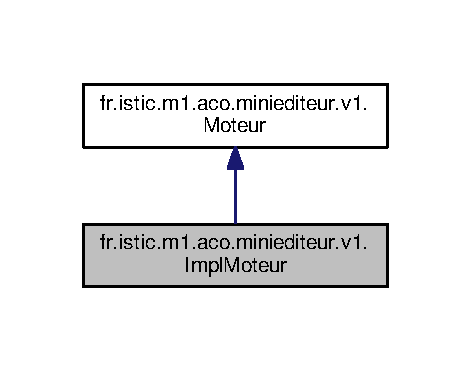
\includegraphics[width=226pt]{classfr_1_1istic_1_1m1_1_1aco_1_1miniediteur_1_1v1_1_1ImplMoteur__inherit__graph}
\end{center}
\end{figure}


Graphe de collaboration de fr.\+istic.\+m1.\+aco.\+miniediteur.\+v1.\+Impl\+Moteur\+:
\nopagebreak
\begin{figure}[H]
\begin{center}
\leavevmode
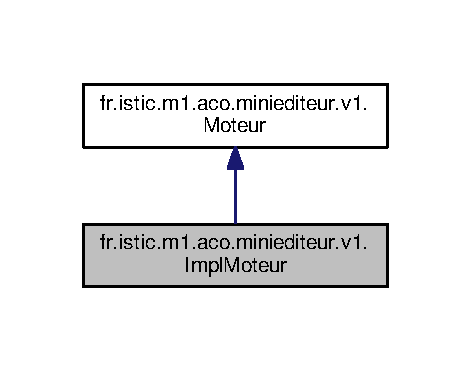
\includegraphics[width=226pt]{classfr_1_1istic_1_1m1_1_1aco_1_1miniediteur_1_1v1_1_1ImplMoteur__coll__graph}
\end{center}
\end{figure}
\subsection*{Fonctions membres publiques}
\begin{DoxyCompactItemize}
\item 
\mbox{\Hypertarget{classfr_1_1istic_1_1m1_1_1aco_1_1miniediteur_1_1v1_1_1ImplMoteur_accc285eb40fcf3dd10d9e759572693b4}\label{classfr_1_1istic_1_1m1_1_1aco_1_1miniediteur_1_1v1_1_1ImplMoteur_accc285eb40fcf3dd10d9e759572693b4}} 
void {\bfseries couper} ()  throws Unsupported\+Operation\+Exception 
\item 
\mbox{\Hypertarget{classfr_1_1istic_1_1m1_1_1aco_1_1miniediteur_1_1v1_1_1ImplMoteur_a8878eeb5dd3b768bf3cdad749eb4bdbe}\label{classfr_1_1istic_1_1m1_1_1aco_1_1miniediteur_1_1v1_1_1ImplMoteur_a8878eeb5dd3b768bf3cdad749eb4bdbe}} 
void {\bfseries copier} ()  throws Unsupported\+Operation\+Exception 
\item 
\mbox{\Hypertarget{classfr_1_1istic_1_1m1_1_1aco_1_1miniediteur_1_1v1_1_1ImplMoteur_aabba2aa78984cb79aa82eec8c357d19b}\label{classfr_1_1istic_1_1m1_1_1aco_1_1miniediteur_1_1v1_1_1ImplMoteur_aabba2aa78984cb79aa82eec8c357d19b}} 
void {\bfseries coller} ()  throws Unsupported\+Operation\+Exception 
\item 
\mbox{\Hypertarget{classfr_1_1istic_1_1m1_1_1aco_1_1miniediteur_1_1v1_1_1ImplMoteur_a28a7d1b3a7e6df691897ccf02f5fc881}\label{classfr_1_1istic_1_1m1_1_1aco_1_1miniediteur_1_1v1_1_1ImplMoteur_a28a7d1b3a7e6df691897ccf02f5fc881}} 
void {\bfseries inserer} (String s)  throws Unsupported\+Operation\+Exception 
\item 
\mbox{\Hypertarget{classfr_1_1istic_1_1m1_1_1aco_1_1miniediteur_1_1v1_1_1ImplMoteur_ac4aa178459855e2a146417d12deb9011}\label{classfr_1_1istic_1_1m1_1_1aco_1_1miniediteur_1_1v1_1_1ImplMoteur_ac4aa178459855e2a146417d12deb9011}} 
void {\bfseries selectionner} (int debut, int fin)  throws Unsupported\+Operation\+Exception 
\end{DoxyCompactItemize}


\subsection{Description détaillée}
Created by 16009566 on 20/10/17. 

La documentation de cette classe a été générée à partir du fichier suivant \+:\begin{DoxyCompactItemize}
\item 
src/fr/istic/m1/aco/miniediteur/v1/Impl\+Moteur.\+java\end{DoxyCompactItemize}

\hypertarget{classfr_1_1istic_1_1m1_1_1aco_1_1miniediteur_1_1v1_1_1Inserer}{}\section{Référence de la classe fr.\+istic.\+m1.\+aco.\+miniediteur.\+v1.\+Inserer}
\label{classfr_1_1istic_1_1m1_1_1aco_1_1miniediteur_1_1v1_1_1Inserer}\index{fr.\+istic.\+m1.\+aco.\+miniediteur.\+v1.\+Inserer@{fr.\+istic.\+m1.\+aco.\+miniediteur.\+v1.\+Inserer}}


Graphe d\textquotesingle{}héritage de fr.\+istic.\+m1.\+aco.\+miniediteur.\+v1.\+Inserer\+:
\nopagebreak
\begin{figure}[H]
\begin{center}
\leavevmode
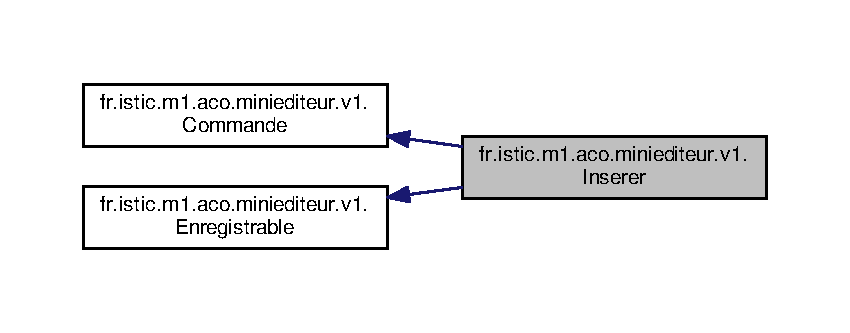
\includegraphics[width=350pt]{classfr_1_1istic_1_1m1_1_1aco_1_1miniediteur_1_1v1_1_1Inserer__inherit__graph}
\end{center}
\end{figure}


Graphe de collaboration de fr.\+istic.\+m1.\+aco.\+miniediteur.\+v1.\+Inserer\+:
\nopagebreak
\begin{figure}[H]
\begin{center}
\leavevmode
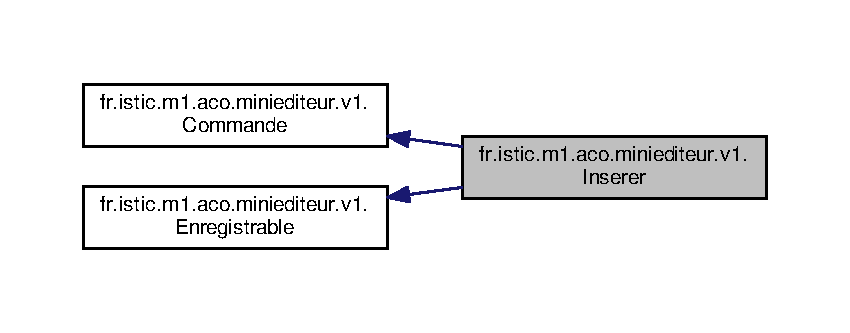
\includegraphics[width=350pt]{classfr_1_1istic_1_1m1_1_1aco_1_1miniediteur_1_1v1_1_1Inserer__coll__graph}
\end{center}
\end{figure}
\subsection*{Fonctions membres publiques}
\begin{DoxyCompactItemize}
\item 
\mbox{\Hypertarget{classfr_1_1istic_1_1m1_1_1aco_1_1miniediteur_1_1v1_1_1Inserer_acbf4c75249a1836789c8ab4dcc7dcb0d}\label{classfr_1_1istic_1_1m1_1_1aco_1_1miniediteur_1_1v1_1_1Inserer_acbf4c75249a1836789c8ab4dcc7dcb0d}} 
void \hyperlink{classfr_1_1istic_1_1m1_1_1aco_1_1miniediteur_1_1v1_1_1Inserer_acbf4c75249a1836789c8ab4dcc7dcb0d}{execute} ()
\begin{DoxyCompactList}\small\item\em Méthode commune aux commandes devant implémenter leur action quand déclenchée par l\textquotesingle{}\hyperlink{interfacefr_1_1istic_1_1m1_1_1aco_1_1miniediteur_1_1v1_1_1IHM}{I\+HM}. \end{DoxyCompactList}\item 
\mbox{\Hypertarget{classfr_1_1istic_1_1m1_1_1aco_1_1miniediteur_1_1v1_1_1Inserer_a4091c321237a04db9509b01e2baf768f}\label{classfr_1_1istic_1_1m1_1_1aco_1_1miniediteur_1_1v1_1_1Inserer_a4091c321237a04db9509b01e2baf768f}} 
\hyperlink{interfacefr_1_1istic_1_1m1_1_1aco_1_1miniediteur_1_1v1_1_1Memento}{Memento} {\bfseries get\+Memento} ()
\item 
\mbox{\Hypertarget{classfr_1_1istic_1_1m1_1_1aco_1_1miniediteur_1_1v1_1_1Inserer_a1978002e0aa031a5293ff3263c49fe94}\label{classfr_1_1istic_1_1m1_1_1aco_1_1miniediteur_1_1v1_1_1Inserer_a1978002e0aa031a5293ff3263c49fe94}} 
void {\bfseries set\+Memento} (\hyperlink{interfacefr_1_1istic_1_1m1_1_1aco_1_1miniediteur_1_1v1_1_1Memento}{Memento} m)
\end{DoxyCompactItemize}


\subsection{Description détaillée}
Created by 16009566 on 13/10/17. 

La documentation de cette classe a été générée à partir du fichier suivant \+:\begin{DoxyCompactItemize}
\item 
src/fr/istic/m1/aco/miniediteur/v1/Inserer.\+java\end{DoxyCompactItemize}

\hypertarget{interfacefr_1_1istic_1_1m1_1_1aco_1_1miniediteur_1_1v1_1_1Memento}{}\section{Référence de l\textquotesingle{}interface fr.\+istic.\+m1.\+aco.\+miniediteur.\+v1.\+Memento}
\label{interfacefr_1_1istic_1_1m1_1_1aco_1_1miniediteur_1_1v1_1_1Memento}\index{fr.\+istic.\+m1.\+aco.\+miniediteur.\+v1.\+Memento@{fr.\+istic.\+m1.\+aco.\+miniediteur.\+v1.\+Memento}}


Graphe d\textquotesingle{}héritage de fr.\+istic.\+m1.\+aco.\+miniediteur.\+v1.\+Memento\+:\nopagebreak
\begin{figure}[H]
\begin{center}
\leavevmode
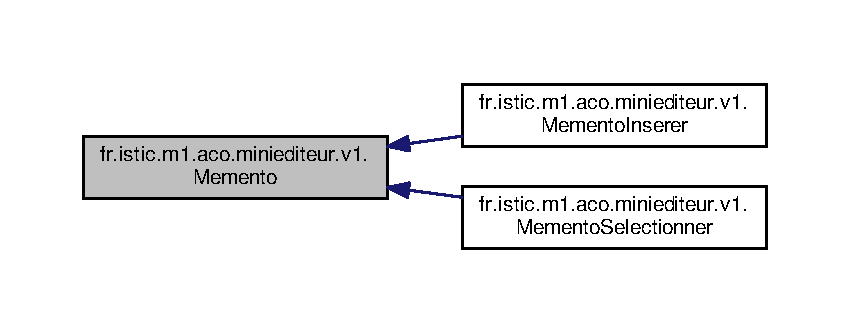
\includegraphics[width=350pt]{interfacefr_1_1istic_1_1m1_1_1aco_1_1miniediteur_1_1v1_1_1Memento__inherit__graph}
\end{center}
\end{figure}


\subsection{Description détaillée}
Created by 16009566 on 13/10/17. 

La documentation de cette interface a été générée à partir du fichier suivant \+:\begin{DoxyCompactItemize}
\item 
src/fr/istic/m1/aco/miniediteur/v1/Memento.\+java\end{DoxyCompactItemize}

\hypertarget{classfr_1_1istic_1_1m1_1_1aco_1_1miniediteur_1_1v1_1_1MementoInserer}{}\section{Référence de la classe fr.\+istic.\+m1.\+aco.\+miniediteur.\+v1.\+Memento\+Inserer}
\label{classfr_1_1istic_1_1m1_1_1aco_1_1miniediteur_1_1v1_1_1MementoInserer}\index{fr.\+istic.\+m1.\+aco.\+miniediteur.\+v1.\+Memento\+Inserer@{fr.\+istic.\+m1.\+aco.\+miniediteur.\+v1.\+Memento\+Inserer}}


Graphe d\textquotesingle{}héritage de fr.\+istic.\+m1.\+aco.\+miniediteur.\+v1.\+Memento\+Inserer\+:
\nopagebreak
\begin{figure}[H]
\begin{center}
\leavevmode
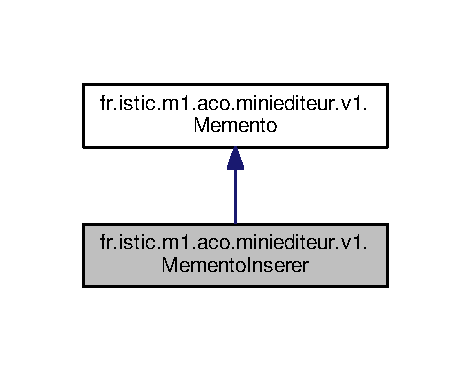
\includegraphics[width=226pt]{classfr_1_1istic_1_1m1_1_1aco_1_1miniediteur_1_1v1_1_1MementoInserer__inherit__graph}
\end{center}
\end{figure}


Graphe de collaboration de fr.\+istic.\+m1.\+aco.\+miniediteur.\+v1.\+Memento\+Inserer\+:
\nopagebreak
\begin{figure}[H]
\begin{center}
\leavevmode
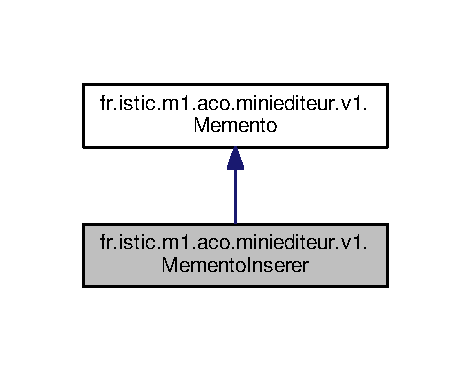
\includegraphics[width=226pt]{classfr_1_1istic_1_1m1_1_1aco_1_1miniediteur_1_1v1_1_1MementoInserer__coll__graph}
\end{center}
\end{figure}
\subsection*{Fonctions membres publiques}
\begin{DoxyCompactItemize}
\item 
\mbox{\Hypertarget{classfr_1_1istic_1_1m1_1_1aco_1_1miniediteur_1_1v1_1_1MementoInserer_a0d639b4f1974085e017b86c98a95ccfc}\label{classfr_1_1istic_1_1m1_1_1aco_1_1miniediteur_1_1v1_1_1MementoInserer_a0d639b4f1974085e017b86c98a95ccfc}} 
{\bfseries Memento\+Inserer} (String str)
\item 
\mbox{\Hypertarget{classfr_1_1istic_1_1m1_1_1aco_1_1miniediteur_1_1v1_1_1MementoInserer_a9aefd3489567d9cdcdb81236d1f99408}\label{classfr_1_1istic_1_1m1_1_1aco_1_1miniediteur_1_1v1_1_1MementoInserer_a9aefd3489567d9cdcdb81236d1f99408}} 
String {\bfseries get\+Text} ()
\end{DoxyCompactItemize}


\subsection{Description détaillée}
Created by 16009566 on 13/10/17. 

La documentation de cette classe a été générée à partir du fichier suivant \+:\begin{DoxyCompactItemize}
\item 
src/fr/istic/m1/aco/miniediteur/v1/Memento\+Inserer.\+java\end{DoxyCompactItemize}

\hypertarget{classfr_1_1istic_1_1m1_1_1aco_1_1miniediteur_1_1v1_1_1MementoSelectionner}{}\section{Référence de la classe fr.\+istic.\+m1.\+aco.\+miniediteur.\+v1.\+Memento\+Selectionner}
\label{classfr_1_1istic_1_1m1_1_1aco_1_1miniediteur_1_1v1_1_1MementoSelectionner}\index{fr.\+istic.\+m1.\+aco.\+miniediteur.\+v1.\+Memento\+Selectionner@{fr.\+istic.\+m1.\+aco.\+miniediteur.\+v1.\+Memento\+Selectionner}}


Graphe d\textquotesingle{}héritage de fr.\+istic.\+m1.\+aco.\+miniediteur.\+v1.\+Memento\+Selectionner\+:\nopagebreak
\begin{figure}[H]
\begin{center}
\leavevmode
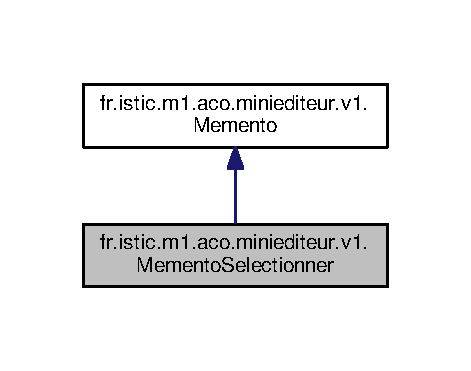
\includegraphics[width=226pt]{classfr_1_1istic_1_1m1_1_1aco_1_1miniediteur_1_1v1_1_1MementoSelectionner__inherit__graph}
\end{center}
\end{figure}


Graphe de collaboration de fr.\+istic.\+m1.\+aco.\+miniediteur.\+v1.\+Memento\+Selectionner\+:\nopagebreak
\begin{figure}[H]
\begin{center}
\leavevmode
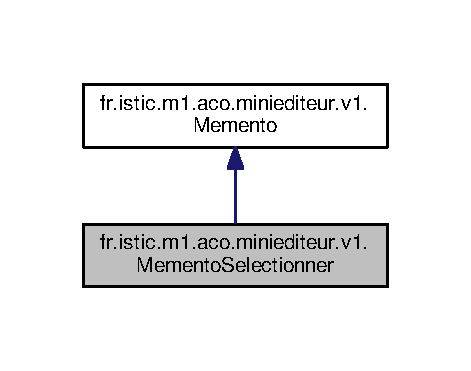
\includegraphics[width=226pt]{classfr_1_1istic_1_1m1_1_1aco_1_1miniediteur_1_1v1_1_1MementoSelectionner__coll__graph}
\end{center}
\end{figure}
\subsection*{Fonctions membres publiques}
\begin{DoxyCompactItemize}
\item 
\mbox{\Hypertarget{classfr_1_1istic_1_1m1_1_1aco_1_1miniediteur_1_1v1_1_1MementoSelectionner_a060ba628c123b1de2d5a4ab0afce96fb}\label{classfr_1_1istic_1_1m1_1_1aco_1_1miniediteur_1_1v1_1_1MementoSelectionner_a060ba628c123b1de2d5a4ab0afce96fb}} 
{\bfseries Memento\+Selectionner} (int debut, int fin)
\item 
\mbox{\Hypertarget{classfr_1_1istic_1_1m1_1_1aco_1_1miniediteur_1_1v1_1_1MementoSelectionner_aa1ce7afca63236c0e5e9730989238871}\label{classfr_1_1istic_1_1m1_1_1aco_1_1miniediteur_1_1v1_1_1MementoSelectionner_aa1ce7afca63236c0e5e9730989238871}} 
int {\bfseries get\+Deb} ()
\item 
\mbox{\Hypertarget{classfr_1_1istic_1_1m1_1_1aco_1_1miniediteur_1_1v1_1_1MementoSelectionner_acb03cb0b6bb4d368379ea46089b16c5f}\label{classfr_1_1istic_1_1m1_1_1aco_1_1miniediteur_1_1v1_1_1MementoSelectionner_acb03cb0b6bb4d368379ea46089b16c5f}} 
int {\bfseries get\+Fin} ()
\end{DoxyCompactItemize}


\subsection{Description détaillée}
Created by 16009566 on 20/10/17. 

La documentation de cette classe a été générée à partir du fichier suivant \+:\begin{DoxyCompactItemize}
\item 
src/fr/istic/m1/aco/miniediteur/v1/Memento\+Selectionner.\+java\end{DoxyCompactItemize}

\hypertarget{interfacefr_1_1istic_1_1m1_1_1aco_1_1miniediteur_1_1v1_1_1Moteur}{}\section{Référence de l\textquotesingle{}interface fr.\+istic.\+m1.\+aco.\+miniediteur.\+v1.\+Moteur}
\label{interfacefr_1_1istic_1_1m1_1_1aco_1_1miniediteur_1_1v1_1_1Moteur}\index{fr.\+istic.\+m1.\+aco.\+miniediteur.\+v1.\+Moteur@{fr.\+istic.\+m1.\+aco.\+miniediteur.\+v1.\+Moteur}}


Graphe d\textquotesingle{}héritage de fr.\+istic.\+m1.\+aco.\+miniediteur.\+v1.\+Moteur\+:\nopagebreak
\begin{figure}[H]
\begin{center}
\leavevmode
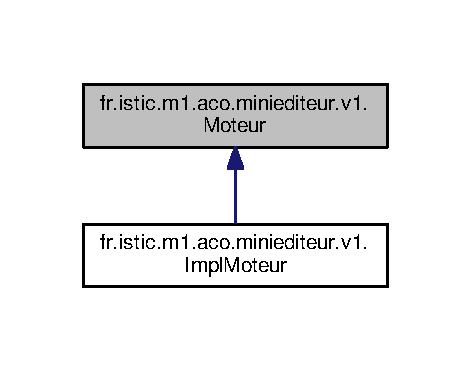
\includegraphics[width=226pt]{interfacefr_1_1istic_1_1m1_1_1aco_1_1miniediteur_1_1v1_1_1Moteur__inherit__graph}
\end{center}
\end{figure}
\subsection*{Fonctions membres publiques}
\begin{DoxyCompactItemize}
\item 
\mbox{\Hypertarget{interfacefr_1_1istic_1_1m1_1_1aco_1_1miniediteur_1_1v1_1_1Moteur_a9848e371756d9a79c6221ddf9a5b9fb0}\label{interfacefr_1_1istic_1_1m1_1_1aco_1_1miniediteur_1_1v1_1_1Moteur_a9848e371756d9a79c6221ddf9a5b9fb0}} 
void {\bfseries couper} ()  throws Unsupported\+Operation\+Exception
\item 
\mbox{\Hypertarget{interfacefr_1_1istic_1_1m1_1_1aco_1_1miniediteur_1_1v1_1_1Moteur_a4a8f8428d290d0243c13e6b694d25660}\label{interfacefr_1_1istic_1_1m1_1_1aco_1_1miniediteur_1_1v1_1_1Moteur_a4a8f8428d290d0243c13e6b694d25660}} 
void {\bfseries copier} ()  throws Unsupported\+Operation\+Exception
\item 
\mbox{\Hypertarget{interfacefr_1_1istic_1_1m1_1_1aco_1_1miniediteur_1_1v1_1_1Moteur_a18ecda9d88a1abaa9721d33b6d012d01}\label{interfacefr_1_1istic_1_1m1_1_1aco_1_1miniediteur_1_1v1_1_1Moteur_a18ecda9d88a1abaa9721d33b6d012d01}} 
void {\bfseries coller} ()  throws Unsupported\+Operation\+Exception
\item 
\mbox{\Hypertarget{interfacefr_1_1istic_1_1m1_1_1aco_1_1miniediteur_1_1v1_1_1Moteur_a68e1c5499dea3f74d6d019efaebde638}\label{interfacefr_1_1istic_1_1m1_1_1aco_1_1miniediteur_1_1v1_1_1Moteur_a68e1c5499dea3f74d6d019efaebde638}} 
void {\bfseries inserer} (String s)  throws Unsupported\+Operation\+Exception
\item 
\mbox{\Hypertarget{interfacefr_1_1istic_1_1m1_1_1aco_1_1miniediteur_1_1v1_1_1Moteur_a5ca7f0486e1037b7549077cb5f3ceb91}\label{interfacefr_1_1istic_1_1m1_1_1aco_1_1miniediteur_1_1v1_1_1Moteur_a5ca7f0486e1037b7549077cb5f3ceb91}} 
void {\bfseries selectionner} (int debut, int fin)  throws Unsupported\+Operation\+Exception
\end{DoxyCompactItemize}


La documentation de cette interface a été générée à partir du fichier suivant \+:\begin{DoxyCompactItemize}
\item 
src/fr/istic/m1/aco/miniediteur/v1/Moteur.\+java\end{DoxyCompactItemize}

\hypertarget{classfr_1_1istic_1_1m1_1_1aco_1_1miniediteur_1_1v1_1_1PressePapier}{}\section{Référence de la classe fr.\+istic.\+m1.\+aco.\+miniediteur.\+v1.\+Presse\+Papier}
\label{classfr_1_1istic_1_1m1_1_1aco_1_1miniediteur_1_1v1_1_1PressePapier}\index{fr.\+istic.\+m1.\+aco.\+miniediteur.\+v1.\+Presse\+Papier@{fr.\+istic.\+m1.\+aco.\+miniediteur.\+v1.\+Presse\+Papier}}


\subsection{Description détaillée}
Created by 16009566 on 20/10/17. 

La documentation de cette classe a été générée à partir du fichier suivant \+:\begin{DoxyCompactItemize}
\item 
src/fr/istic/m1/aco/miniediteur/v1/Presse\+Papier.\+java\end{DoxyCompactItemize}

\hypertarget{classfr_1_1istic_1_1m1_1_1aco_1_1miniediteur_1_1v1_1_1Refaire}{}\section{Référence de la classe fr.\+istic.\+m1.\+aco.\+miniediteur.\+v1.\+Refaire}
\label{classfr_1_1istic_1_1m1_1_1aco_1_1miniediteur_1_1v1_1_1Refaire}\index{fr.\+istic.\+m1.\+aco.\+miniediteur.\+v1.\+Refaire@{fr.\+istic.\+m1.\+aco.\+miniediteur.\+v1.\+Refaire}}


Graphe d\textquotesingle{}héritage de fr.\+istic.\+m1.\+aco.\+miniediteur.\+v1.\+Refaire\+:\nopagebreak
\begin{figure}[H]
\begin{center}
\leavevmode
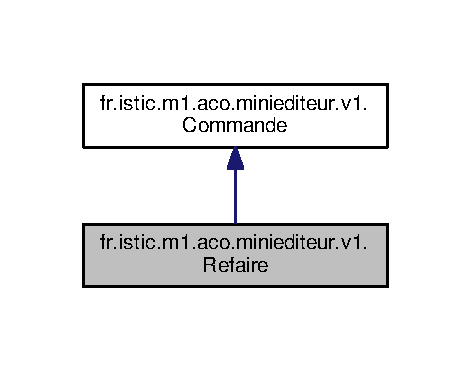
\includegraphics[width=226pt]{classfr_1_1istic_1_1m1_1_1aco_1_1miniediteur_1_1v1_1_1Refaire__inherit__graph}
\end{center}
\end{figure}


Graphe de collaboration de fr.\+istic.\+m1.\+aco.\+miniediteur.\+v1.\+Refaire\+:\nopagebreak
\begin{figure}[H]
\begin{center}
\leavevmode
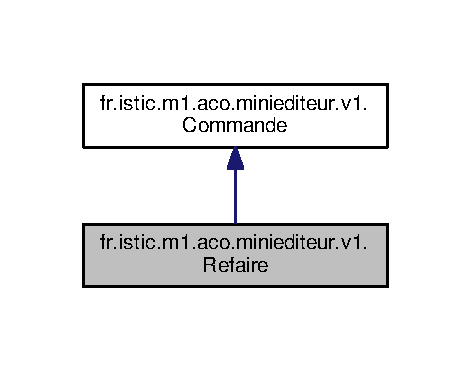
\includegraphics[width=226pt]{classfr_1_1istic_1_1m1_1_1aco_1_1miniediteur_1_1v1_1_1Refaire__coll__graph}
\end{center}
\end{figure}
\subsection*{Fonctions membres publiques}
\begin{DoxyCompactItemize}
\item 
\mbox{\Hypertarget{classfr_1_1istic_1_1m1_1_1aco_1_1miniediteur_1_1v1_1_1Refaire_accb0d09315abed5674ea85477a530819}\label{classfr_1_1istic_1_1m1_1_1aco_1_1miniediteur_1_1v1_1_1Refaire_accb0d09315abed5674ea85477a530819}} 
void \hyperlink{classfr_1_1istic_1_1m1_1_1aco_1_1miniediteur_1_1v1_1_1Refaire_accb0d09315abed5674ea85477a530819}{execute} ()
\begin{DoxyCompactList}\small\item\em Opération commune aux commandes devant implémenter leur action quand déclenchée par l\textquotesingle{}\hyperlink{interfacefr_1_1istic_1_1m1_1_1aco_1_1miniediteur_1_1v1_1_1IHM}{I\+HM}. \end{DoxyCompactList}\end{DoxyCompactItemize}


\subsection{Description détaillée}
Created by 16009566 on 20/10/17. 

La documentation de cette classe a été générée à partir du fichier suivant \+:\begin{DoxyCompactItemize}
\item 
src/fr/istic/m1/aco/miniediteur/v1/Refaire.\+java\end{DoxyCompactItemize}

\hypertarget{classfr_1_1istic_1_1m1_1_1aco_1_1miniediteur_1_1v1_1_1Rejouer}{}\section{Référence de la classe fr.\+istic.\+m1.\+aco.\+miniediteur.\+v1.\+Rejouer}
\label{classfr_1_1istic_1_1m1_1_1aco_1_1miniediteur_1_1v1_1_1Rejouer}\index{fr.\+istic.\+m1.\+aco.\+miniediteur.\+v1.\+Rejouer@{fr.\+istic.\+m1.\+aco.\+miniediteur.\+v1.\+Rejouer}}


Graphe d\textquotesingle{}héritage de fr.\+istic.\+m1.\+aco.\+miniediteur.\+v1.\+Rejouer\+:
\nopagebreak
\begin{figure}[H]
\begin{center}
\leavevmode
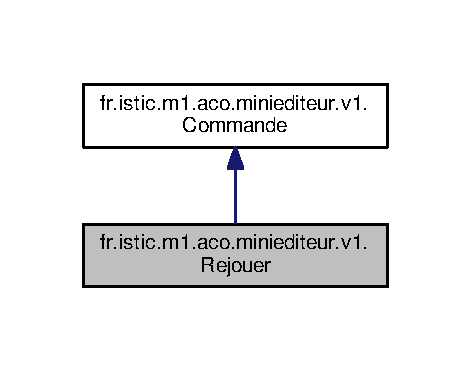
\includegraphics[width=226pt]{classfr_1_1istic_1_1m1_1_1aco_1_1miniediteur_1_1v1_1_1Rejouer__inherit__graph}
\end{center}
\end{figure}


Graphe de collaboration de fr.\+istic.\+m1.\+aco.\+miniediteur.\+v1.\+Rejouer\+:
\nopagebreak
\begin{figure}[H]
\begin{center}
\leavevmode
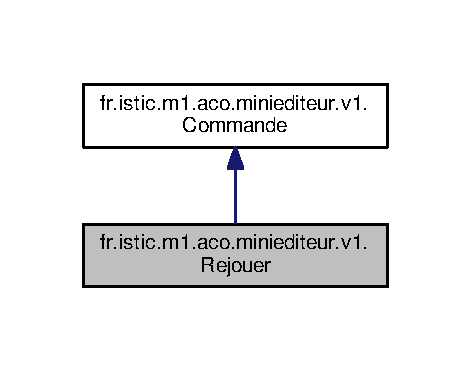
\includegraphics[width=226pt]{classfr_1_1istic_1_1m1_1_1aco_1_1miniediteur_1_1v1_1_1Rejouer__coll__graph}
\end{center}
\end{figure}
\subsection*{Fonctions membres publiques}
\begin{DoxyCompactItemize}
\item 
\mbox{\Hypertarget{classfr_1_1istic_1_1m1_1_1aco_1_1miniediteur_1_1v1_1_1Rejouer_a4c2093ae315b9520fa94a1f058a4d815}\label{classfr_1_1istic_1_1m1_1_1aco_1_1miniediteur_1_1v1_1_1Rejouer_a4c2093ae315b9520fa94a1f058a4d815}} 
void \hyperlink{classfr_1_1istic_1_1m1_1_1aco_1_1miniediteur_1_1v1_1_1Rejouer_a4c2093ae315b9520fa94a1f058a4d815}{execute} ()
\begin{DoxyCompactList}\small\item\em Méthode commune aux commandes devant implémenter leur action quand déclenchée par l\textquotesingle{}\hyperlink{interfacefr_1_1istic_1_1m1_1_1aco_1_1miniediteur_1_1v1_1_1IHM}{I\+HM}. \end{DoxyCompactList}\end{DoxyCompactItemize}


\subsection{Description détaillée}
Created by 16009566 on 13/10/17. 

La documentation de cette classe a été générée à partir du fichier suivant \+:\begin{DoxyCompactItemize}
\item 
src/fr/istic/m1/aco/miniediteur/v1/Rejouer.\+java\end{DoxyCompactItemize}

\hypertarget{classfr_1_1istic_1_1m1_1_1aco_1_1miniediteur_1_1v1_1_1Selection}{}\section{Référence de la classe fr.\+istic.\+m1.\+aco.\+miniediteur.\+v1.\+Selection}
\label{classfr_1_1istic_1_1m1_1_1aco_1_1miniediteur_1_1v1_1_1Selection}\index{fr.\+istic.\+m1.\+aco.\+miniediteur.\+v1.\+Selection@{fr.\+istic.\+m1.\+aco.\+miniediteur.\+v1.\+Selection}}


\subsection{Description détaillée}
Created by 16009566 on 20/10/17. 

La documentation de cette classe a été générée à partir du fichier suivant \+:\begin{DoxyCompactItemize}
\item 
src/fr/istic/m1/aco/miniediteur/v1/Selection.\+java\end{DoxyCompactItemize}

\hypertarget{classfr_1_1istic_1_1m1_1_1aco_1_1miniediteur_1_1v1_1_1Selectionner}{}\section{Référence de la classe fr.\+istic.\+m1.\+aco.\+miniediteur.\+v1.\+Selectionner}
\label{classfr_1_1istic_1_1m1_1_1aco_1_1miniediteur_1_1v1_1_1Selectionner}\index{fr.\+istic.\+m1.\+aco.\+miniediteur.\+v1.\+Selectionner@{fr.\+istic.\+m1.\+aco.\+miniediteur.\+v1.\+Selectionner}}


Graphe d\textquotesingle{}héritage de fr.\+istic.\+m1.\+aco.\+miniediteur.\+v1.\+Selectionner\+:
\nopagebreak
\begin{figure}[H]
\begin{center}
\leavevmode
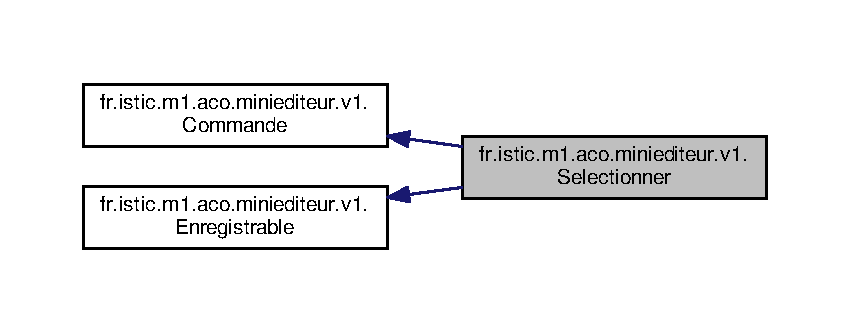
\includegraphics[width=350pt]{classfr_1_1istic_1_1m1_1_1aco_1_1miniediteur_1_1v1_1_1Selectionner__inherit__graph}
\end{center}
\end{figure}


Graphe de collaboration de fr.\+istic.\+m1.\+aco.\+miniediteur.\+v1.\+Selectionner\+:
\nopagebreak
\begin{figure}[H]
\begin{center}
\leavevmode
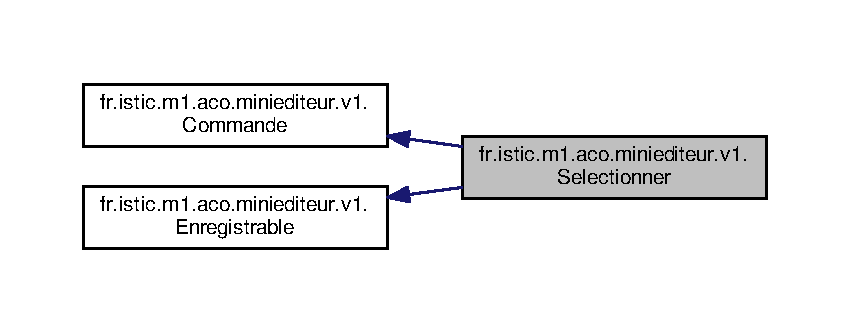
\includegraphics[width=350pt]{classfr_1_1istic_1_1m1_1_1aco_1_1miniediteur_1_1v1_1_1Selectionner__coll__graph}
\end{center}
\end{figure}
\subsection*{Fonctions membres publiques}
\begin{DoxyCompactItemize}
\item 
\mbox{\Hypertarget{classfr_1_1istic_1_1m1_1_1aco_1_1miniediteur_1_1v1_1_1Selectionner_a746abe8d1a13dbb084f37d4b67fa1261}\label{classfr_1_1istic_1_1m1_1_1aco_1_1miniediteur_1_1v1_1_1Selectionner_a746abe8d1a13dbb084f37d4b67fa1261}} 
void \hyperlink{classfr_1_1istic_1_1m1_1_1aco_1_1miniediteur_1_1v1_1_1Selectionner_a746abe8d1a13dbb084f37d4b67fa1261}{execute} ()
\begin{DoxyCompactList}\small\item\em Opération commune aux commandes devant implémenter leur action quand déclenchée par l\textquotesingle{}\hyperlink{interfacefr_1_1istic_1_1m1_1_1aco_1_1miniediteur_1_1v1_1_1IHM}{I\+HM}. \end{DoxyCompactList}\item 
\hyperlink{interfacefr_1_1istic_1_1m1_1_1aco_1_1miniediteur_1_1v1_1_1Memento}{Memento} \hyperlink{classfr_1_1istic_1_1m1_1_1aco_1_1miniediteur_1_1v1_1_1Selectionner_a93bb9249ee51f501735f6b40d77dc3f3}{get\+Memento} ()
\begin{DoxyCompactList}\small\item\em Opération permettant d\textquotesingle{}obtenir une copie de l\textquotesingle{}état d\textquotesingle{}une opération requérant une sauvegarde pour pouvoir être refaire ultérieurement. \end{DoxyCompactList}\item 
void \hyperlink{classfr_1_1istic_1_1m1_1_1aco_1_1miniediteur_1_1v1_1_1Selectionner_a80d7d18546f239290919a9e602405ffd}{set\+Memento} (\hyperlink{interfacefr_1_1istic_1_1m1_1_1aco_1_1miniediteur_1_1v1_1_1Memento}{Memento} m)
\begin{DoxyCompactList}\small\item\em Opération permettant de réinitialiser la commande par rapport à un état précédent donné sous la forme d\textquotesingle{}un \hyperlink{interfacefr_1_1istic_1_1m1_1_1aco_1_1miniediteur_1_1v1_1_1Memento}{Memento}. \end{DoxyCompactList}\end{DoxyCompactItemize}


\subsection{Description détaillée}
Created by 16009566 on 13/10/17. 

\subsection{Documentation des fonctions membres}
\mbox{\Hypertarget{classfr_1_1istic_1_1m1_1_1aco_1_1miniediteur_1_1v1_1_1Selectionner_a93bb9249ee51f501735f6b40d77dc3f3}\label{classfr_1_1istic_1_1m1_1_1aco_1_1miniediteur_1_1v1_1_1Selectionner_a93bb9249ee51f501735f6b40d77dc3f3}} 
\index{fr\+::istic\+::m1\+::aco\+::miniediteur\+::v1\+::\+Selectionner@{fr\+::istic\+::m1\+::aco\+::miniediteur\+::v1\+::\+Selectionner}!get\+Memento@{get\+Memento}}
\index{get\+Memento@{get\+Memento}!fr\+::istic\+::m1\+::aco\+::miniediteur\+::v1\+::\+Selectionner@{fr\+::istic\+::m1\+::aco\+::miniediteur\+::v1\+::\+Selectionner}}
\subsubsection{\texorpdfstring{get\+Memento()}{getMemento()}}
{\footnotesize\ttfamily \hyperlink{interfacefr_1_1istic_1_1m1_1_1aco_1_1miniediteur_1_1v1_1_1Memento}{Memento} fr.\+istic.\+m1.\+aco.\+miniediteur.\+v1.\+Selectionner.\+get\+Memento (\begin{DoxyParamCaption}{ }\end{DoxyParamCaption})}



Opération permettant d\textquotesingle{}obtenir une copie de l\textquotesingle{}état d\textquotesingle{}une opération requérant une sauvegarde pour pouvoir être refaire ultérieurement. 

\begin{DoxyReturn}{Renvoie}
Une instance implémentant \hyperlink{interfacefr_1_1istic_1_1m1_1_1aco_1_1miniediteur_1_1v1_1_1Memento}{Memento} qui est une copie de l\textquotesingle{}état de la commande. 
\end{DoxyReturn}


Implémente \hyperlink{interfacefr_1_1istic_1_1m1_1_1aco_1_1miniediteur_1_1v1_1_1Enregistrable_aadf173c765d103d3924bbb688c45abb6}{fr.\+istic.\+m1.\+aco.\+miniediteur.\+v1.\+Enregistrable}.

\mbox{\Hypertarget{classfr_1_1istic_1_1m1_1_1aco_1_1miniediteur_1_1v1_1_1Selectionner_a80d7d18546f239290919a9e602405ffd}\label{classfr_1_1istic_1_1m1_1_1aco_1_1miniediteur_1_1v1_1_1Selectionner_a80d7d18546f239290919a9e602405ffd}} 
\index{fr\+::istic\+::m1\+::aco\+::miniediteur\+::v1\+::\+Selectionner@{fr\+::istic\+::m1\+::aco\+::miniediteur\+::v1\+::\+Selectionner}!set\+Memento@{set\+Memento}}
\index{set\+Memento@{set\+Memento}!fr\+::istic\+::m1\+::aco\+::miniediteur\+::v1\+::\+Selectionner@{fr\+::istic\+::m1\+::aco\+::miniediteur\+::v1\+::\+Selectionner}}
\subsubsection{\texorpdfstring{set\+Memento()}{setMemento()}}
{\footnotesize\ttfamily void fr.\+istic.\+m1.\+aco.\+miniediteur.\+v1.\+Selectionner.\+set\+Memento (\begin{DoxyParamCaption}\item[{\hyperlink{interfacefr_1_1istic_1_1m1_1_1aco_1_1miniediteur_1_1v1_1_1Memento}{Memento}}]{m }\end{DoxyParamCaption})}



Opération permettant de réinitialiser la commande par rapport à un état précédent donné sous la forme d\textquotesingle{}un \hyperlink{interfacefr_1_1istic_1_1m1_1_1aco_1_1miniediteur_1_1v1_1_1Memento}{Memento}. 


\begin{DoxyParams}{Paramètres}
{\em m} & un \hyperlink{interfacefr_1_1istic_1_1m1_1_1aco_1_1miniediteur_1_1v1_1_1Memento}{Memento} décrivant un état précédent de la commande sur lequel revenir \\
\hline
\end{DoxyParams}


Implémente \hyperlink{interfacefr_1_1istic_1_1m1_1_1aco_1_1miniediteur_1_1v1_1_1Enregistrable_a949bb6784743800c2d743def265f41b1}{fr.\+istic.\+m1.\+aco.\+miniediteur.\+v1.\+Enregistrable}.



La documentation de cette classe a été générée à partir du fichier suivant \+:\begin{DoxyCompactItemize}
\item 
src/fr/istic/m1/aco/miniediteur/v1/Selectionner.\+java\end{DoxyCompactItemize}

\hypertarget{classfr_1_1istic_1_1m1_1_1aco_1_1miniediteur_1_1v1_1_1Stopper}{}\section{Référence de la classe fr.\+istic.\+m1.\+aco.\+miniediteur.\+v1.\+Stopper}
\label{classfr_1_1istic_1_1m1_1_1aco_1_1miniediteur_1_1v1_1_1Stopper}\index{fr.\+istic.\+m1.\+aco.\+miniediteur.\+v1.\+Stopper@{fr.\+istic.\+m1.\+aco.\+miniediteur.\+v1.\+Stopper}}


Graphe d\textquotesingle{}héritage de fr.\+istic.\+m1.\+aco.\+miniediteur.\+v1.\+Stopper\+:\nopagebreak
\begin{figure}[H]
\begin{center}
\leavevmode
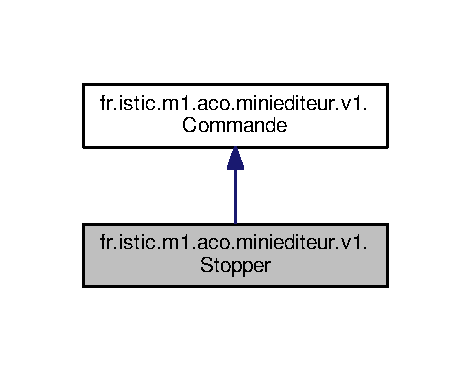
\includegraphics[width=226pt]{classfr_1_1istic_1_1m1_1_1aco_1_1miniediteur_1_1v1_1_1Stopper__inherit__graph}
\end{center}
\end{figure}


Graphe de collaboration de fr.\+istic.\+m1.\+aco.\+miniediteur.\+v1.\+Stopper\+:\nopagebreak
\begin{figure}[H]
\begin{center}
\leavevmode
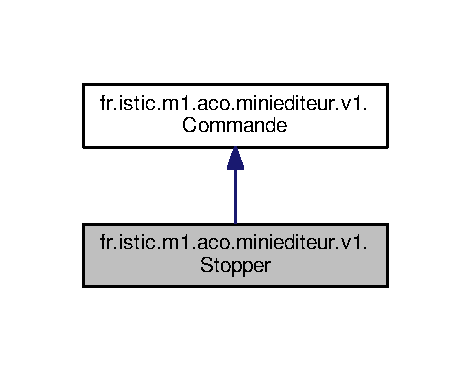
\includegraphics[width=226pt]{classfr_1_1istic_1_1m1_1_1aco_1_1miniediteur_1_1v1_1_1Stopper__coll__graph}
\end{center}
\end{figure}
\subsection*{Fonctions membres publiques}
\begin{DoxyCompactItemize}
\item 
\mbox{\Hypertarget{classfr_1_1istic_1_1m1_1_1aco_1_1miniediteur_1_1v1_1_1Stopper_a39d1f6428e1fb70e179c45537e41a20e}\label{classfr_1_1istic_1_1m1_1_1aco_1_1miniediteur_1_1v1_1_1Stopper_a39d1f6428e1fb70e179c45537e41a20e}} 
void \hyperlink{classfr_1_1istic_1_1m1_1_1aco_1_1miniediteur_1_1v1_1_1Stopper_a39d1f6428e1fb70e179c45537e41a20e}{execute} ()
\begin{DoxyCompactList}\small\item\em Opération commune aux commandes devant implémenter leur action quand déclenchée par l\textquotesingle{}\hyperlink{interfacefr_1_1istic_1_1m1_1_1aco_1_1miniediteur_1_1v1_1_1IHM}{I\+HM}. \end{DoxyCompactList}\end{DoxyCompactItemize}


\subsection{Description détaillée}
Created by 16009566 on 13/10/17. 

La documentation de cette classe a été générée à partir du fichier suivant \+:\begin{DoxyCompactItemize}
\item 
src/fr/istic/m1/aco/miniediteur/v1/Stopper.\+java\end{DoxyCompactItemize}

\chapter{Documentation des fichiers}
\hypertarget{Coller_8java}{}\section{Référence du fichier src/fr/istic/m1/aco/miniediteur/v1/\+Coller.java}
\label{Coller_8java}\index{src/fr/istic/m1/aco/miniediteur/v1/\+Coller.\+java@{src/fr/istic/m1/aco/miniediteur/v1/\+Coller.\+java}}
\subsection*{Classes}
\begin{DoxyCompactItemize}
\item 
class \hyperlink{classfr_1_1istic_1_1m1_1_1aco_1_1miniediteur_1_1v1_1_1Coller}{fr.\+istic.\+m1.\+aco.\+miniediteur.\+v1.\+Coller}
\begin{DoxyCompactList}\small\item\em Classe contrôlant le fonctionnement de la fonctionnalité permettant de \hyperlink{classfr_1_1istic_1_1m1_1_1aco_1_1miniediteur_1_1v1_1_1Coller}{Coller} dans un \char`\"{}copié-\/collé\char`\"{}. \end{DoxyCompactList}\end{DoxyCompactItemize}
\subsection*{Paquetages}
\begin{DoxyCompactItemize}
\item 
package \hyperlink{namespacefr_1_1istic_1_1m1_1_1aco_1_1miniediteur_1_1v1}{fr.\+istic.\+m1.\+aco.\+miniediteur.\+v1}
\end{DoxyCompactItemize}


\subsection{Description détaillée}
\begin{DoxyAuthor}{Auteur}
Dorian \char`\"{}\+Aexelion\char`\"{} D\+U\+M\+A\+N\+G\+ET 

Corentin \char`\"{}\+Heartbroken-\/\+Git\char`\"{} C\+HÉ\+D\+O\+T\+AL 
\end{DoxyAuthor}
\begin{DoxyCopyright}{Copyright}
L\+P\+R\+AB 
\end{DoxyCopyright}

\hypertarget{Commande_8java}{}\section{Référence du fichier src/fr/istic/m1/aco/miniediteur/v1/\+Commande.java}
\label{Commande_8java}\index{src/fr/istic/m1/aco/miniediteur/v1/\+Commande.\+java@{src/fr/istic/m1/aco/miniediteur/v1/\+Commande.\+java}}
\subsection*{Classes}
\begin{DoxyCompactItemize}
\item 
interface \hyperlink{interfacefr_1_1istic_1_1m1_1_1aco_1_1miniediteur_1_1v1_1_1Commande}{fr.\+istic.\+m1.\+aco.\+miniediteur.\+v1.\+Commande}
\begin{DoxyCompactList}\small\item\em Interface décrivant une commande déclenchée par une action sur l\textquotesingle{}\hyperlink{interfacefr_1_1istic_1_1m1_1_1aco_1_1miniediteur_1_1v1_1_1IHM}{I\+HM} de l\textquotesingle{}Utilisateur. \end{DoxyCompactList}\end{DoxyCompactItemize}
\subsection*{Paquetages}
\begin{DoxyCompactItemize}
\item 
package \hyperlink{namespacefr_1_1istic_1_1m1_1_1aco_1_1miniediteur_1_1v1}{fr.\+istic.\+m1.\+aco.\+miniediteur.\+v1}
\end{DoxyCompactItemize}


\subsection{Description détaillée}
\begin{DoxyAuthor}{Auteur}
Dorian \char`\"{}\+Aexelion\char`\"{} D\+U\+M\+A\+N\+G\+ET 

Corentin \char`\"{}\+Heartbroken-\/\+Git\char`\"{} C\+HÉ\+D\+O\+T\+AL 
\end{DoxyAuthor}
\begin{DoxyCopyright}{Copyright}
L\+P\+R\+AB 1.\+0 
\end{DoxyCopyright}

\hypertarget{Copier_8java}{}\section{Référence du fichier src/fr/istic/m1/aco/miniediteur/v1/\+Copier.java}
\label{Copier_8java}\index{src/fr/istic/m1/aco/miniediteur/v1/\+Copier.\+java@{src/fr/istic/m1/aco/miniediteur/v1/\+Copier.\+java}}
\subsection*{Classes}
\begin{DoxyCompactItemize}
\item 
class \hyperlink{classfr_1_1istic_1_1m1_1_1aco_1_1miniediteur_1_1v1_1_1Copier}{fr.\+istic.\+m1.\+aco.\+miniediteur.\+v1.\+Copier}
\begin{DoxyCompactList}\small\item\em Classe contrôlant le fonctionnement de la fonctionnalité permettant de \hyperlink{classfr_1_1istic_1_1m1_1_1aco_1_1miniediteur_1_1v1_1_1Copier}{Copier} dans un \char`\"{}copié-\/collé\char`\"{}. \end{DoxyCompactList}\end{DoxyCompactItemize}
\subsection*{Paquetages}
\begin{DoxyCompactItemize}
\item 
package \hyperlink{namespacefr_1_1istic_1_1m1_1_1aco_1_1miniediteur_1_1v1}{fr.\+istic.\+m1.\+aco.\+miniediteur.\+v1}
\end{DoxyCompactItemize}


\subsection{Description détaillée}
\begin{DoxyAuthor}{Auteur}
Dorian \char`\"{}\+Aexelion\char`\"{} D\+U\+M\+A\+N\+G\+ET 

Corentin \char`\"{}\+Heartbroken-\/\+Git\char`\"{} C\+HÉ\+D\+O\+T\+AL 
\end{DoxyAuthor}
\begin{DoxyCopyright}{Copyright}
L\+P\+R\+AB 1.\+0 
\end{DoxyCopyright}

\hypertarget{Couper_8java}{}\section{Référence du fichier src/fr/istic/m1/aco/miniediteur/v1/\+Couper.java}
\label{Couper_8java}\index{src/fr/istic/m1/aco/miniediteur/v1/\+Couper.\+java@{src/fr/istic/m1/aco/miniediteur/v1/\+Couper.\+java}}
\subsection*{Classes}
\begin{DoxyCompactItemize}
\item 
class \hyperlink{classfr_1_1istic_1_1m1_1_1aco_1_1miniediteur_1_1v1_1_1Couper}{fr.\+istic.\+m1.\+aco.\+miniediteur.\+v1.\+Couper}
\begin{DoxyCompactList}\small\item\em Classe contrôlant le fonctionnement de la fonctionnalité permettant de \hyperlink{classfr_1_1istic_1_1m1_1_1aco_1_1miniediteur_1_1v1_1_1Copier}{Copier} dans un \char`\"{}copié-\/collé\char`\"{}. \end{DoxyCompactList}\end{DoxyCompactItemize}
\subsection*{Paquetages}
\begin{DoxyCompactItemize}
\item 
package \hyperlink{namespacefr_1_1istic_1_1m1_1_1aco_1_1miniediteur_1_1v1}{fr.\+istic.\+m1.\+aco.\+miniediteur.\+v1}
\end{DoxyCompactItemize}


\subsection{Description détaillée}
\begin{DoxyAuthor}{Auteur}
Dorian \char`\"{}\+Aexelion\char`\"{} D\+U\+M\+A\+N\+G\+ET 

Corentin \char`\"{}\+Heartbroken-\/\+Git\char`\"{} C\+HÉ\+D\+O\+T\+AL 
\end{DoxyAuthor}
\begin{DoxyCopyright}{Copyright}
L\+P\+R\+AB 1.\+0 
\end{DoxyCopyright}

\hypertarget{Defaire_8java}{}\section{Référence du fichier src/fr/istic/m1/aco/miniediteur/v1/\+Defaire.java}
\label{Defaire_8java}\index{src/fr/istic/m1/aco/miniediteur/v1/\+Defaire.\+java@{src/fr/istic/m1/aco/miniediteur/v1/\+Defaire.\+java}}
\subsection*{Classes}
\begin{DoxyCompactItemize}
\item 
class \hyperlink{classfr_1_1istic_1_1m1_1_1aco_1_1miniediteur_1_1v1_1_1Defaire}{fr.\+istic.\+m1.\+aco.\+miniediteur.\+v1.\+Defaire}
\begin{DoxyCompactList}\small\item\em Classe contrôlant le fonctionnement de la fonctionnalité permettant de Défaire dans un \char`\"{}défaire-\/refaire\char`\"{}. \end{DoxyCompactList}\end{DoxyCompactItemize}
\subsection*{Paquetages}
\begin{DoxyCompactItemize}
\item 
package \hyperlink{namespacefr_1_1istic_1_1m1_1_1aco_1_1miniediteur_1_1v1}{fr.\+istic.\+m1.\+aco.\+miniediteur.\+v1}
\end{DoxyCompactItemize}


\subsection{Description détaillée}
\begin{DoxyAuthor}{Auteur}
Dorian \char`\"{}\+Aexelion\char`\"{} D\+U\+M\+A\+N\+G\+ET 

Corentin \char`\"{}\+Heartbroken-\/\+Git\char`\"{} C\+HÉ\+D\+O\+T\+AL 
\end{DoxyAuthor}
\begin{DoxyCopyright}{Copyright}
L\+P\+R\+AB 1.\+0 
\end{DoxyCopyright}

\hypertarget{Demarrer_8java}{}\section{Référence du fichier src/fr/istic/m1/aco/miniediteur/v1/\+Demarrer.java}
\label{Demarrer_8java}\index{src/fr/istic/m1/aco/miniediteur/v1/\+Demarrer.\+java@{src/fr/istic/m1/aco/miniediteur/v1/\+Demarrer.\+java}}
\subsection*{Classes}
\begin{DoxyCompactItemize}
\item 
class \hyperlink{classfr_1_1istic_1_1m1_1_1aco_1_1miniediteur_1_1v1_1_1Demarrer}{fr.\+istic.\+m1.\+aco.\+miniediteur.\+v1.\+Demarrer}
\begin{DoxyCompactList}\small\item\em Classe contrôlant le fonctionnement de la fonctionnalité permettant de débuter l\textquotesingle{}enregistrement d\textquotesingle{}une macro. \end{DoxyCompactList}\end{DoxyCompactItemize}
\subsection*{Paquetages}
\begin{DoxyCompactItemize}
\item 
package \hyperlink{namespacefr_1_1istic_1_1m1_1_1aco_1_1miniediteur_1_1v1}{fr.\+istic.\+m1.\+aco.\+miniediteur.\+v1}
\end{DoxyCompactItemize}


\subsection{Description détaillée}
\begin{DoxyAuthor}{Auteur}
Dorian \char`\"{}\+Aexelion\char`\"{} D\+U\+M\+A\+N\+G\+ET 

Corentin \char`\"{}\+Heartbroken-\/\+Git\char`\"{} C\+HÉ\+D\+O\+T\+AL 
\end{DoxyAuthor}
\begin{DoxyCopyright}{Copyright}
L\+P\+R\+AB 1.\+0 
\end{DoxyCopyright}

\hypertarget{Enregistrable_8java}{}\section{Référence du fichier src/fr/istic/m1/aco/miniediteur/v1/\+Enregistrable.java}
\label{Enregistrable_8java}\index{src/fr/istic/m1/aco/miniediteur/v1/\+Enregistrable.\+java@{src/fr/istic/m1/aco/miniediteur/v1/\+Enregistrable.\+java}}
\subsection*{Classes}
\begin{DoxyCompactItemize}
\item 
interface \hyperlink{interfacefr_1_1istic_1_1m1_1_1aco_1_1miniediteur_1_1v1_1_1Enregistrable}{fr.\+istic.\+m1.\+aco.\+miniediteur.\+v1.\+Enregistrable}
\begin{DoxyCompactList}\small\item\em Interface décrivant des actions pouvant faire l\textquotesingle{}objet d\textquotesingle{}un enregistrement pour une macro. \end{DoxyCompactList}\end{DoxyCompactItemize}
\subsection*{Paquetages}
\begin{DoxyCompactItemize}
\item 
package \hyperlink{namespacefr_1_1istic_1_1m1_1_1aco_1_1miniediteur_1_1v1}{fr.\+istic.\+m1.\+aco.\+miniediteur.\+v1}
\end{DoxyCompactItemize}


\subsection{Description détaillée}
\begin{DoxyAuthor}{Auteur}
Dorian \char`\"{}\+Aexelion\char`\"{} D\+U\+M\+A\+N\+G\+ET 

Corentin \char`\"{}\+Heartbroken-\/\+Git\char`\"{} C\+HÉ\+D\+O\+T\+AL 
\end{DoxyAuthor}
\begin{DoxyCopyright}{Copyright}
L\+P\+R\+AB 1.\+0 
\end{DoxyCopyright}

\hypertarget{Enregistreur_8java}{}\section{Référence du fichier src/fr/istic/m1/aco/miniediteur/v1/\+Enregistreur.java}
\label{Enregistreur_8java}\index{src/fr/istic/m1/aco/miniediteur/v1/\+Enregistreur.\+java@{src/fr/istic/m1/aco/miniediteur/v1/\+Enregistreur.\+java}}
\subsection*{Classes}
\begin{DoxyCompactItemize}
\item 
interface \hyperlink{interfacefr_1_1istic_1_1m1_1_1aco_1_1miniediteur_1_1v1_1_1Enregistreur}{fr.\+istic.\+m1.\+aco.\+miniediteur.\+v1.\+Enregistreur}
\begin{DoxyCompactList}\small\item\em Interface décrivant les actions d\textquotesingle{}enregistrement de macros. \end{DoxyCompactList}\end{DoxyCompactItemize}
\subsection*{Paquetages}
\begin{DoxyCompactItemize}
\item 
package \hyperlink{namespacefr_1_1istic_1_1m1_1_1aco_1_1miniediteur_1_1v1}{fr.\+istic.\+m1.\+aco.\+miniediteur.\+v1}
\end{DoxyCompactItemize}


\subsection{Description détaillée}
\begin{DoxyAuthor}{Auteur}
Dorian \char`\"{}\+Aexelion\char`\"{} D\+U\+M\+A\+N\+G\+ET 

Corentin \char`\"{}\+Heartbroken-\/\+Git\char`\"{} C\+HÉ\+D\+O\+T\+AL 
\end{DoxyAuthor}
\begin{DoxyCopyright}{Copyright}
L\+P\+R\+AB 1.\+0 
\end{DoxyCopyright}

\hypertarget{GestionnaireDefaireRefaire_8java}{}\section{Référence du fichier src/fr/istic/m1/aco/miniediteur/v1/\+Gestionnaire\+Defaire\+Refaire.java}
\label{GestionnaireDefaireRefaire_8java}\index{src/fr/istic/m1/aco/miniediteur/v1/\+Gestionnaire\+Defaire\+Refaire.\+java@{src/fr/istic/m1/aco/miniediteur/v1/\+Gestionnaire\+Defaire\+Refaire.\+java}}
\subsection*{Classes}
\begin{DoxyCompactItemize}
\item 
interface \hyperlink{interfacefr_1_1istic_1_1m1_1_1aco_1_1miniediteur_1_1v1_1_1GestionnaireDefaireRefaire}{fr.\+istic.\+m1.\+aco.\+miniediteur.\+v1.\+Gestionnaire\+Defaire\+Refaire}
\begin{DoxyCompactList}\small\item\em Interface décrivant les mécanismes permettant d\textquotesingle{}annuler une action de l\textquotesingle{}utilisateur et éventuellement de la refaire. \end{DoxyCompactList}\end{DoxyCompactItemize}
\subsection*{Paquetages}
\begin{DoxyCompactItemize}
\item 
package \hyperlink{namespacefr_1_1istic_1_1m1_1_1aco_1_1miniediteur_1_1v1}{fr.\+istic.\+m1.\+aco.\+miniediteur.\+v1}
\end{DoxyCompactItemize}


\subsection{Description détaillée}
\begin{DoxyAuthor}{Auteur}
Dorian \char`\"{}\+Aexelion\char`\"{} D\+U\+M\+A\+N\+G\+ET 

Corentin \char`\"{}\+Heartbroken-\/\+Git\char`\"{} C\+HÉ\+D\+O\+T\+AL 
\end{DoxyAuthor}
\begin{DoxyCopyright}{Copyright}
L\+P\+R\+AB 1.\+0 
\end{DoxyCopyright}

\hypertarget{IHM_8java}{}\section{Référence du fichier src/fr/istic/m1/aco/miniediteur/v1/\+I\+HM.java}
\label{IHM_8java}\index{src/fr/istic/m1/aco/miniediteur/v1/\+I\+H\+M.\+java@{src/fr/istic/m1/aco/miniediteur/v1/\+I\+H\+M.\+java}}
\subsection*{Classes}
\begin{DoxyCompactItemize}
\item 
interface \hyperlink{interfacefr_1_1istic_1_1m1_1_1aco_1_1miniediteur_1_1v1_1_1IHM}{fr.\+istic.\+m1.\+aco.\+miniediteur.\+v1.\+I\+HM}
\begin{DoxyCompactList}\small\item\em Interface décrivant les opérations requises pour toutes les interfaces hommes machines. \end{DoxyCompactList}\end{DoxyCompactItemize}
\subsection*{Paquetages}
\begin{DoxyCompactItemize}
\item 
package \hyperlink{namespacefr_1_1istic_1_1m1_1_1aco_1_1miniediteur_1_1v1}{fr.\+istic.\+m1.\+aco.\+miniediteur.\+v1}
\end{DoxyCompactItemize}


\subsection{Description détaillée}
\begin{DoxyAuthor}{Auteur}
Dorian \char`\"{}\+Aexelion\char`\"{} D\+U\+M\+A\+N\+G\+ET 

Corentin \char`\"{}\+Heartbroken-\/\+Git\char`\"{} C\+HÉ\+D\+O\+T\+AL 
\end{DoxyAuthor}
\begin{DoxyCopyright}{Copyright}
L\+P\+R\+AB 1.\+0 
\end{DoxyCopyright}

\hypertarget{Inserer_8java}{}\section{Référence du fichier src/fr/istic/m1/aco/miniediteur/v1/\+Inserer.java}
\label{Inserer_8java}\index{src/fr/istic/m1/aco/miniediteur/v1/\+Inserer.\+java@{src/fr/istic/m1/aco/miniediteur/v1/\+Inserer.\+java}}
\subsection*{Classes}
\begin{DoxyCompactItemize}
\item 
class \hyperlink{classfr_1_1istic_1_1m1_1_1aco_1_1miniediteur_1_1v1_1_1Inserer}{fr.\+istic.\+m1.\+aco.\+miniediteur.\+v1.\+Inserer}
\begin{DoxyCompactList}\small\item\em Classe contrôlant le fonctionnement de la commande d\textquotesingle{}insertion de texte dans l\textquotesingle{}éditeur. \end{DoxyCompactList}\end{DoxyCompactItemize}
\subsection*{Paquetages}
\begin{DoxyCompactItemize}
\item 
package \hyperlink{namespacefr_1_1istic_1_1m1_1_1aco_1_1miniediteur_1_1v1}{fr.\+istic.\+m1.\+aco.\+miniediteur.\+v1}
\end{DoxyCompactItemize}


\subsection{Description détaillée}
\begin{DoxyAuthor}{Auteur}
Dorian \char`\"{}\+Aexelion\char`\"{} D\+U\+M\+A\+N\+G\+ET 

Corentin \char`\"{}\+Heartbroken-\/\+Git\char`\"{} C\+HÉ\+D\+O\+T\+AL 
\end{DoxyAuthor}
\begin{DoxyCopyright}{Copyright}
L\+P\+R\+AB 1.\+0 
\end{DoxyCopyright}

%--- End generated contents ---

% Index
\backmatter
\newpage
\phantomsection
\clearemptydoublepage
\addcontentsline{toc}{chapter}{Index}
\printindex

\end{document}
